\setchapterpreamble[u]{\vspace*{-3\baselineskip}\margintoc}
\chapter{Turbulent Frameworks}
\labch{2}

\section{General Introduction}
\subsection{The concept of turbulence}
\newthought{What is} Turbulence, how can, and should it be represented ?
Initially, turbulence was associated to a chaotic and irregular
motion of people.
During the Age of Renaissance in Italy, Leonardo da Vinci was the first to
apply this term to the apparently random motion of a fluid giving a detailed
description of a turbulent waterfall. He highlighted, as a painter, 
the important role played by the coherent structures in the flow, such as the
vortices, and understood that even though the microscopic features of a turbulent fluid change, the macroscopic characteristics keep organizing themselves in the same manner every time the phenomenon is reproduced. 
\begin{marginfigure}[2cm]
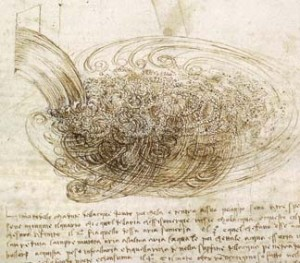
\includegraphics[width=\linewidth]{2/leo.png}
\caption{Undated sketch of a turbulent waterfall made by Leonardo da Vinci.}
\end{marginfigure}
After Leonardo, many scientists have been interested in this phenomenon, and as many were the definitions of turbulence proposed. Nevertheless, none of these definitions has been accepted as a unique, formal and satisfying definition of turbulence. However, there is consensus on the characteristics shown by turbulent systems :
\begin{itemize}[leftmargin=1.5cm]
\item disorganised, seemingly random behaviour;
\item dynamics non-repeatable but statistics repeatable;
\item many excited modes/degrees of freedom involved;
\item scale-invariance/self-similarity;
\item state far from equilibrium;
\item enhanced diffusion and dissipation.
\end{itemize}
The irregularity or random character of all turbulent flows makes a determinis-
tic approach to the turbulence problem nearly intractable. Indeed, even though
the governing equation of fluid dynamics, that is, the Navier-Stokes equation,
is a deterministic equation, it contains non-linear terms, which become domi-
nant as turbulence develops, leading to an intractable analytical resolution of
this equation. Thus, statistical methods have been adopted for the study of
fully developed turbulence, which find their basis on the phenomenological
description of this process. 


Turbulence is an ubiquitous state of fluid flow in which the flow variables, such as velocity or temperature, exhibit complex variation in both space and time. It is a phenomenon widely observed in both terrestrial
environments such as the atmosphere and the oceans and extraterrestrial environments such as stellar interiors, the ISM and the intra-cluster medium in galaxy clusters. 
An important difference between
terrestrial and astrophysical turbulence is that while terrestrial turbulence is always a flow of a neutral fluid, such as water or air, astrophysical turbulence almost always concerns the motion of an ionized fluid threaded
by a dynamically important magnetic field. Turbulence in the ISM is an important example of astrophysical turbulence, and has significant consequences on ISM physics and chemistry.
We will propose a self-contained presentation of the vast turbulence problem, with particular emphasis on issues relevant to energy dissipation and intermittency.
\begin{marginfigure}[0.5cm]
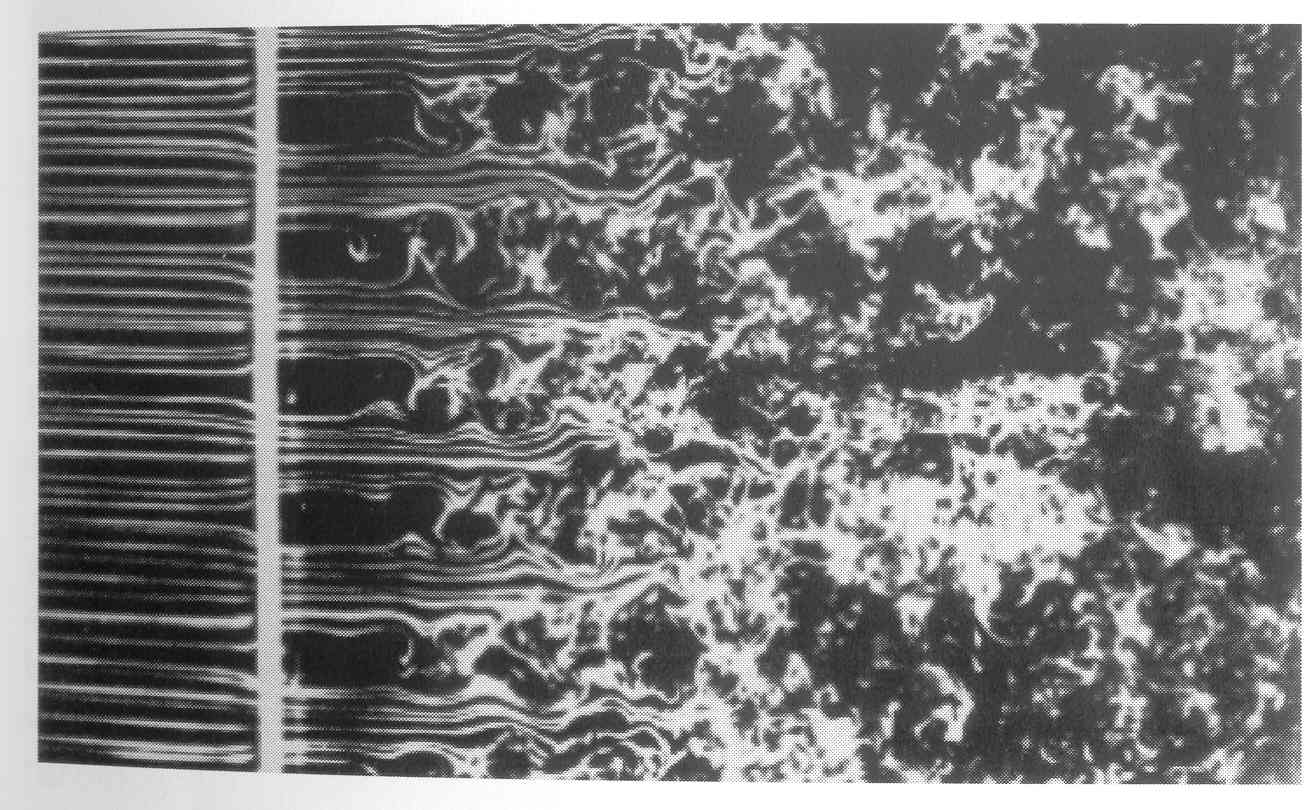
\includegraphics[width=\linewidth]{2/turb1.png}\vspace{.25\baselineskip}
\includegraphics[width=\linewidth]{2/turb2.jpg}\vspace{.25\baselineskip}
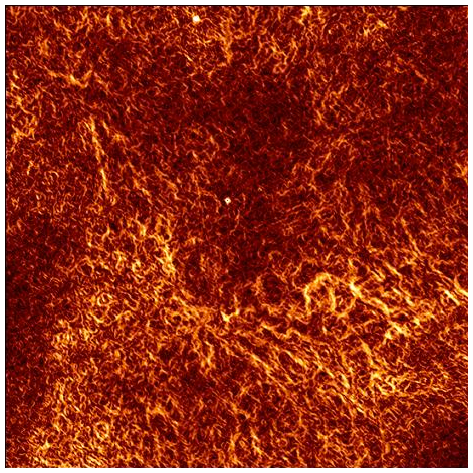
\includegraphics[width=\linewidth]{2/turb3.png}\vspace{.25\baselineskip}

\includegraphics[width=\linewidth]{2/turb4.png}
\caption{Examples of turbulent flows. From top to bottom Classical laboratory experiment of homogeneous isotropic
turbulence generated behind a grid [Corke et al., 1982].
Phytoplankton bloom reveals turbulent ocean currents, an example of geophysical turbulence [Signorini and McClain, 2009].  Turbulence
in the interstellar medium as revealed by the gradient of linear polarization [Gaensler et al., 2011]. Current density magnitude in a high resolution numerical experiment of homogeneous isotropic
magnetohydrodynamic turbulence [G. Momferratos, unpublished].}
\end{marginfigure}
Turbulent flows lie at the interface between order and chaos: although individual realizations of an experiment flow variables can exhibit chaotic variation, there often exists predictable behavior in the statistical sense,
if a sufficiently large number of physical experiments is considered. This important property has led to the development of a statistical theory, which is fundamentally based on the notion of an ensemble average: an experiment is repeated a large number of times in such a way that although the initial and boundary conditions are macroscopically identical, small perturbations in them lead to a sample of turbulent flow fields from which an average can be extracted. In practice, the ensemble average is often replaced with an average
with respect to space or time, assuming a corresponding ergodic hypothesis.
This variability between different experiments with macroscopically identical initial conditions is known as sensitive dependence on initial conditions and is a signature of chaotic dynamics of nonlinear systems. 

This phenomenon has been studied extensively in the context of low-dimensional dynamical systems typically described by ordinary differential equations. Turbulence, being a phenomenon extended in both space and time, has in principle an infinite number of degrees of freedom and is the prototypical example of spatio-temporal chaos, where a very large number of degrees of freedom interact non-linearly.
But how much are these degrees of freedom excited, as a function of their characteristic scale? Contrary to other complex phenomena studied in statistical physics, in turbulence there is no clear-cut separation
of scales. Energy as a function of scale is rather characterized by a continuous spectrum, which can be accounted for by simple phenomenological assumptions. Turbulence is thus a multiscale phenomenon, where different degrees of freedom, each having a specific scale, interact with each other to produce a continuous
energy spectrum. 

This interaction between structures at different scales leads to the phenomenological picture of the energy cascade. Energy is injected at large scales, either by a driving force or by appropriate boundary conditions. At
scales much smaller than the energy containing scale, but still large enough so that viscosity is unimportant, nonlinear interaction between modes transfer energy from large to small scales in a conservative way; this range of scales is called the inertial range. Finally, energy reaches scales small enough such that viscosity cannot be neglected, and is dissipated into heat there; this range of scales is known as the dissipative range.
Energy dissipation is however not uniformly distributed in space and time, but is characterized by strong localized bursts alternating between larger quiescent regions. This property of fluid turbulence, known as intermittency, has important theoretical as well as practical consequences. On the theoretical side, it is capable of modifying the phenomenological picture based on the energy cascade in a nontrivial way. On the practical side, the intermittency of the energy dissipation rate is capable of heating the interstellar medium
above the threshold of certain important chemical reactions, thus activating new chemical routes.

\subsection{Interstellar turbulence}
After a few early propositions that did not catch on [von Weizsäcker 1951],
the omnipresence of turbulence in the interstellar medium has been slowly
recognized starting from the 80’s. Its role is still a subject of debates today,
but its presence and importance is now clearly established.
We now give a quick overview of the observational evidences of turbulence
in the ISM, of the probable sources of kinetic energy initiating the turbulent
cascade, and of the various roles that turbulence can play in different envi-
ronments.
\newthought{Observational} evidences of turbulence in the ISM have been increasing more and more in the past years. 
The first argument in favor of a turbulent ISM comes from estimates of the
Reynolds number based on the observed velocity dispersion of clouds. The
resulting Reynolds number are of the order of $10^7$ . In addition, the velocity
dispersions are actually supersonic, so that interstellar turbulence is probably highly compressible. As the gas in the CNM is also partially ionized and
permeated by a magnetic field of a few micro-gauss, non-ideal MHD processes are most likely also at play, so that several dissipation processes work
in parallel (shocks, viscous shear, resistivity and ambipolar diffusion).
Observations of scaling laws between the velocity dispersion and the cloud
size on one hand, and between the cloud mass and the cloud size on the other
hand [Larson 1981], reminiscent of those found in Kolmogorov theory, have been interpreted as evidences of turbulence. 
\begin{marginfigure}
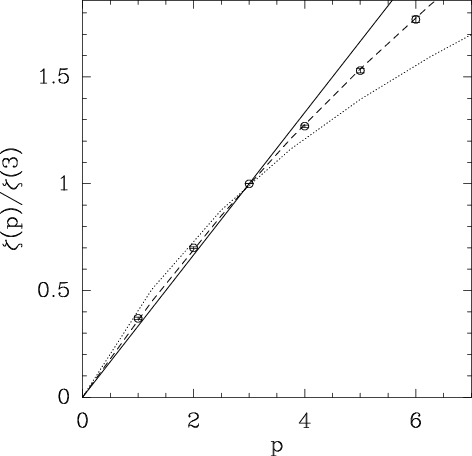
\includegraphics[width=\linewidth]{2/ism.png}
\caption{Structure function exponents for 12 CO observations of Polaris (Hily-Blant
et al. 2008). Solid line: predictions of the Kolmogorov theory of 1941
(no intermittency), dashed line: log-Poisson model of She and Leveque
[1994] for incompressible turbulence, dotted line: predictions of Boldyrev
et al. [2002] for supersonic turbulence. Taken from Hily-Blant et al.
[2008]}
\label{fig:2-ismturbulence}
\end{marginfigure}
Those scaling laws have been confirmed and extended by later studies (e.g. Heyer and Brunt 2004). Power spectra have also been derived from observations, and show a power
law behavior over a large range of scales, with exponents comparable to the
predictions of the Kolmogorov theory. Such spectra have been determined
from a variety of observations: HI emission (Miville-Deschênes et al. 2003),
HI absorption (Deshpande et al. 2000), dust emission (Miville-Deschênes et al.
2010), the electronic density measured from interstellar scintillation (Armstrong et al. 1995), and $^{12}CO$ and $^{13}CO$ emission (Bensch et al. 2001). The
interpretation of these exponents remains difficult as the observables do not
trace the velocity fields directly. A particularly striking evidence of turbulence is the transition in slopes found by Elmegreen et al. [2001] in the HI
spectrum of the large Magellanic Cloud when reaching scales comparable to
the thickness of the HI layer, as expected for the transition from 3D to 2D
turbulence. 

Finally, a third type of evidence of turbulence in the ISM comes from the
measurement of the velocity increment statistics, inferred from the centroid
velocity of line profiles (e.g, Hily-Blant et al. 2008, Hily-Blant and Falgarone 2009). These reveal the non-gaussianity expected from the intermittency of
the turbulence cascade (see Sect.), and the structure exponent derived
from those PDF are surprisingly close to the the predictions of She and Leveque [1994] for incompressible turbulence, as shown on Figure \ref{fig:2-ismturbulence}. Moreover,
the extreme values forming the non-gaussian wings of the PDF correspond to coherent elongated structures with high shear, resembling vortices or shear
layers (Falgarone et al. [2009]).
More evidences are compiled in the reviews by Elmegreen and Scalo [2004]
and Hennebelle and Falgarone [2012]. A recurrent surprise from those evidences is that many results seem to agree well with the prediction for classical incompressible turbulence despite the MHD and incompressible nature expected for interstellar turbulence.

\newthought{Energy sources} are rather scattered : no global trend appears for the energy transfer rate for scales from $10^2$ to $10^{-2}$ pc, and the average value is also consistent [Henebelle and Falgarone 2012], with the one observed in HI gas ($ 2 \times 10^{-25} erg.cm^{-3 }.s ^{-1 }$). As the turbulent motions decay typically in one turnover time (1 Myr for a pc sized cloud and a km.s${-1}$ velocity dispersion), this energy has to be continuously replenished. The question of the origin of this energy remains
open. Several injection mechanisms have been identified, but their relative
importance remains debated.
They can be grouped into stellar sources (supernovae, protostellar wind, O
star winds, super-bubbles expansion), galactic rotation (spiral shock, instabilities due to the differential rotation), and cloud accretion. The uniformity of
the dissipation rates across molecular clouds and the absence of characteristic
scale in their spectrum could point to an external source of energy at scales
larger than the clouds.
It is usually estimated that supernovae and super-bubble expansion are the
dominant energy sources, but other sources could also provide the required
energy more locally (e.g., accretion onto a cloud, Klessen and Hennebelle
[2010]).
An important question is the type of forcing that those sources create, in
term of compressible or solenoidal modes. Indeed, compressible modes tend
to dissipate in large shocks, while solenoidal energy is more prone to undergo
a turbulent cascade.
A more detailed discussion of the energy sources of turbulence can be
found in Elmegreen and Scalo [2004] and Hennebelle and Falgarone [2012].

\newthought{The role} of turbulence of the ISM is unquestionably important, in many different aspects.
For more details see the reviews by Elmegreen et al. [2001] and Scalo
and Elmegreen [2004].
One of the first proposed effects of turbulence is to shape and support
the structure of the ISM. The hierarchical structure of the ISM is interpreted
as a result of compressible turbulence, while the vertical density profile of
the galactic disk requires a dynamical pressure much larger than the thermal
pressure. Turbulent pressure has also been proposed as a support mechanism
for clouds that could slow down the collapse, but numerical studies show
that turbulence tends to disrupt and fragment clouds more than to support
them statically. This turbulent fragmentation process is of great potential
importance for star formation.

One well studied effect of turbulence is to enhance the diffusion of passive
contaminants in the flow. In the ISM, this effect has been invoked for several
distinct problems. One is the observed homogeneity of metals in the galaxy.
Estimates comparing the timescales of supernova ejection of metals and of
reincorporation of metals into new generations of stars show that in the absence of an enhanced mixing mechanism, the distribution of metals should
be very spotty. 

Turbulent transport allows faster mixing and homogenization
of the heavy elements in the ISM, as required by the observations.
Turbulent mixing has also been advocated to explain some aspects of the
chemical composition of the CNM, such as the presence of CO in diffuse gas
insufficiently shielded from radiation, or the presence of atomic hydrogen
inside molecular clouds. However, other mechanisms could explain these observations. Moreover, the estimation of the efficiency of turbulent mixing for
species whose chemistry is controlled by photodissociation is not straightforward. Usual mixing length theory does not apply without adaptation in this
case, as it assumes that a fluid element conserves its chemical composition
while being transported until it reaches the smallest scales of the turbulent
cascade where molecular mixing can take place. Photodissociation will of
course quickly change the composition of the fluid element as soon as its
position is modified. Turbulence also plays a role in the scattering and acceleration of cosmic rays. 

\subsection{Turbulent chemistry}
The energy contained in the interstellar turbulence is dissipated at the end of
the cascade. The absence of cut-off in the observed power spectra shows that
the dissipative scales are not resolved by modern instruments, as expected
from simple estimates (the dissipative scale is of the order of a few AU for
typical diffuse medium conditions). As this dissipation is extremely intermittent, it is expected to create localized and temporary hot spots in which endothermic chemistry
can be activated by the dissipated energy. We discuss here observational
evidences of this mechanism and the models that have been developed to
account for this effect.

\newthought{CH+,SH+ and H2} are very present molecules in the diffuse ISM. $CH^+$ is one of the first interstellar molecules to have been observed in absorption. Yet, conditions in the diffuse CNM in which it is ubiquitously observed
are too cold for the very endothermic reaction 
$$C^+ + H_2 \rightarrow CH^+ + H\quad (4640 K).$$
More recently detected, $SH^+$ is similarly problematic. These observations
have been confirmed and improved many times since the first detection of
these molecules (e.g., Godard et al. [2012]), and still contradict the predictions
of usual PDR-type models, where the chemical dynamics is driven by the UV
radiation field. As the discrepancy mainly concerns molecules with very endothermic formation, this points towards another energy source acting in a
small fraction of the volume, so that the other observables are dominated by
the contribution of the large inactive volume and conform to the predictions
of the PDR models. Thus, the origin of those molecules could be explained
by the intermittent dissipation of energy that occurs at small scales.

Another evidence of this mechanism is the observation by FUSE of significant amounts of rotationally excited $H_2$ on diffuse lines of sight (e.g., Gry
et al. [2002], Lacour et al. [2005]). This excited H 2 in the diffuse ISM has also been observed in emission by Falgarone et al. [2005]. The radiation field
is too weak in these region to cause such levels of excitation by pumping
and cascades, and the gas temperature inferred from the first levels of $H_2$ is
too low to explain the observed populations of the $J > 2$ levels. This again
points towards the presence on the line of sight of a small fraction of high
temperature gas, in which those levels can be collisionaly excited.
Finally, the observed CO abundances on diffuse lines of sight remain one
order of magnitude above the predictions of PDR models (Levrier et al. 2012).
As CO can be formed through the reaction chain 
$$CH^+ - CH_2^+ - CH_3^+ - HCO^+ - CO $$
initiated by the endothermic formation of $CH^+$ , the mechanism described
above to explain the abundance of $CH^+$ could also explain the abundance of
$CO$.

\newthought{Modeling the }interstellar turbulent chemistry remains a major topic. 
The first tentative to explain the abundance of $CH^+$ by a localized dissipation
event was published by Elitzur and Watson [1978], in the form of a shock
originating from the HII region surrounding the observed star. Their model
reproduced the observations of the time, by reaching a sufficiently high gas
temperature to trigger the endothermic reactions.
In a series of paper (Draine and Katz 1986a,b, Draine 1986), Bruce Draine
proposed that the magnetic continuous shocks which he had presented earlier (Draine 1980) could activate the endothermic reaction due to suprathermal collisions caused by ion-neutral drift in the magnetic precursor. A lower
gas temperature was thus required, which could avoid the overproduction of
OH compared to previous models.

This kind of models was later further developed by Flower and Pineau des
Forets [1998]. The ubiquitous presence of $CH^+$ raised the question of the
likelihood of the presence of a single strong shock on every line of sight. This
led Gredel et al. [2002] to propose a model in which a distribution of low
velocity shocks could explain the observations.

In parallel, another kind of dissipative structure was proposed by Joulain
et al. [1998]. In this model, a MHD vortex was proposed to represent the
small scale dissipative structures of MHD turbulence, and the endothermic
formation of CH + was triggered by the ion-neutral drift, similarly to the
shock models. This model was later further developed by Godard et al. [2009],
in which the importance of the cooling phase following the dissipation event
was demonstrated, and the contributions of the dissipative structures, the
cooling gas and the quiescent gas were mixed to model the observation of a
line of sight. The model was shown to reproduce the observations of $CH^+$ ,
$SH^+$ , $CO$ and $H_2$ (and several other tracers).

While these models reproduce in great detail one dissipative structure, the
statistical treatment remains rudimentary. The intermittency of the dissipation is reduced to a binary vision (quiescent gas, and dissipative structures with a single intensity), and the statistics of the Lagrangian history of a fluid
element is not investigated. For instance, whether a particle that just experienced
a dissipative structure has the time to return to the quiescent state before
experiencing another dissipation event.


\section{Governing theoretical models}
\subsection{Incompressible hydrodynamics}
\newthought{Hydrodynamics} of a neutral fluid govern turbulence via the Navier-Stokes equation [Landau-Lifschitz 1987]
\begin{equation}
    \partial_t\mathbf{u}+(\mathbf{u}\cdot\boldsymbol{\nabla})\mathbf{u}=-\boldsymbol{\nabla}\tilde{p}+\nu\nabla^2\mathbf{u}\;,
\end{equation}
whith $\nu=\mu/\rho$ is the kinematic viscosity, $\rho$ the constant mass density, and $\tilde{p}=p/\rho$ the reduced pressure. The incompressibility condition of the velocity field $\mathbf{u}$ can be written as
\begin{equation}
    \nabla\cdot\mathbf{u}=0.
\end{equation}
If the velocity is rescaled by a reference velocity $U$ , spatial coordinates are rescaled by a reference length $L$ and the time coordinate is rescaled by $L/U$, the Navier-Stokes equation remains unchanged except from the substitution of the viscosity $\nu$ with the inverse of the Reynolds number :
\begin{equation}
    \nu^{-1}\longrightarrow \mathcal{R}_e=\frac{UL}{\nu}
\end{equation}
Two flows in domains which are geometrically similar are identical if their Reynolds number are equal. From a physical point of view, the Reynolds number measures the relative importance of the nonlinear advection term $(\mathbf{u}\cdot\boldsymbol{\nabla})\mathbf{u}$ with respect to the viscous term $\nu\nabla^2\mathbf{u}$. A flow with very high Reynolds number \sidenote{A flow with low Reynolds number is a smooth laminar
flow dominated by viscosity. As the Reynolds number is increased, successive instabilities take place and the laminar flow gradually transitions to turbulence.}, presumably an asymptotic state, is known as \emph{fully developed turbulence}. The quadratic nonlinear term, the second term on the left hand side of equation (1), can be identified as the source of the complexity of turbulence. As we will see below, this term is responsible for the interactions
that take place between different scales of the flow.
In incompressible flows, the reduced pressure is not a true dynamical variable, but simply an agent enforcing the incompressibility condition. This can be seen by taking the divergence of equation (1), keeping in mind that the velocity field is solenoidal. One gets the following Poisson equation for the pressure :
\begin{equation}
    \nabla^2\tilde{p}-\partial_iu_j\partial_ju_i=-\partial_i\partial_j(u_iu_j)
\end{equation}
This Poisson equation is an elliptic equation, and this has the important consequence that a local change in the velocity field is propagated instantaneously across the whole flow field through the pressure term. In physical terms, this corresponds to an infinite sound velocity.
Using standard vector identities, one can rewrite the Navier-Stokes equation in rotational form,
\begin{equation}
    \partial_t\mathbf{u}+\boldsymbol{\omega}\times\mathbf{u}=-\nabla\left(\tilde{p}+\frac{1}{2}\mathbf{u}^2\right)+\nu\nabla^2\mathbf{u}, 
\end{equation}
where $\boldsymbol{\omega}=\boldsymbol{\nabla}\times\mathbf{u}$ is the vorticity, a measure of the local rotation rate of the fluid. Taking the curl of this
equation, one obtains an evolution equation for the vorticity
\begin{equation}
    \partial_t\boldsymbol{\omega}=\nabla\times(\mathbf{u}\times\boldsymbol{\omega})+\nu\nabla^2\mathbf{u}
\end{equation}
This is equivalent to using the description 
\begin{equation}
    \partial_t\boldsymbol{\omega}+(\mathbf{u}\cdot\boldsymbol{\nabla})\boldsymbol{\omega}=\frac{D\boldsymbol{\omega}}{Dt}=(\boldsymbol{\omega}\cdot\boldsymbol{\nabla})\mathbf{u}+\nu\nabla^2\boldsymbol{\omega}
\end{equation}
Thus, as the vorticity vector is transported, it is stretched by velocity gradients and diffused by viscosity. This can be interpreted by considering a line $L$ moving with the fluid, with $\delta\ell$ an element on this line. If $\mathbf{v}$ is the velocity of the fluid at one end of the line, say $x$, then the velocity at $x+\delta\ell$ is $\mathbf{v}+(\delta\ell\cdot\boldsymbol{\nabla})\mathbf{u}$. That means, in a time interval $dt$, the line element $\delta\ell$ changes by $dt(\delta\ell\cdot\boldsymbol{\nabla}\mathbf{u}$; i.e,
\begin{equation}
    \frac{D}{Dt}\delta\ell=(\delta\ell\cdot\boldsymbol{\nabla})\mathbf{u}
\end{equation}
and, if we neglect viscous effects, the evolution of the vectors $\delta\ell$ and $\boldsymbol{\omega}$ are given by identical formulae. It follows that if these two vectors are initially in the same direction, they will remain parallel, and the ratio of their moduli will remain constant. 
If we define the vortex lines as the integral curves of the vorticity field,
ie. the solutions of the system of ordinary differential equations
\begin{equation}
    \frac{d\mathbf{r}}{dt}=\boldsymbol{\omega}(\mathbf{r},t)
\end{equation}
wo fluid particles will always be on the same vortex line, and the value of $|\boldsymbol{\omega}|$ will be proportional to the distance between the particles.
This vortex-stretching process is the fundamental mechanism for the transfer of energy from large to small scales in three-dimensional incompressible hydrodynamic turbulence. It is also the primary source of difference between three-dimensional and two-dimensional turbulence, as the term $(\boldsymbol{\omega}\cdot\nabla)\mathbf{u}$ is identically zero in the latter case, the vorticity vector being by definition perpendicular to the plane where $\mathbf{u}$ lies.

It is possible to investigate the role of the nonlinear term on scale interactions by considering the Navier-Stokes equation (1) in Fourier space:
\begin{equation}
    \mathbf{u}(\mathbf{x})=\int_\mathbb{R}\mathbf{u}(\mathbf{k})\exp(i\mathbf{k}\cdot\mathbf{x})d\mathbf{k}
\end{equation}
By this transformation, the velocity field is decomposed into plane waves of wavevector $\mathbf{k}$, which are completely localized in wavenumber space. It is the most simple way to separate the different contributions to
the velocity field coming from different scales and study their interactions.
Eliminating the pressure term from (4), the spectral form of the N-S equation becomes 
\begin{equation}
    \partial_tu_i(\mathbf{k})+\nu k^2u_i(\mathbf{k})=k_iP_{ij}(\mathbf{k})\int_{\mathbf{k}=\mathbf{p}+\mathbf{q}}u_i(\mathbf{q})+u_j(\mathbf{p})d\mathbf{p}d\mathbf{q}
\end{equation}
Where the projection operator,
\begin{equation}
    P_{ij}(\mathbf{k})=\delta_{ij}-\frac{k_ik_j}{k^2},
\end{equation}
ensures the conservation of incompressibility. 
The scale interaction mediated by the nonlinear term now appears as the right hand side of equation (11). The nonlinear term, which is local in physical space, is non-local in Fourier space, effectively a convolution integral. Two perturbations with wavevectors p and q interact to excite a perturbation with wavevector k, but only if these three wavevectors form a triangle: k = p + q. Although this form of the Navier-Stokes equation clearly shows the existence of scale interactions, it provides no information on their locality or non-locality in scale. It also provides no information on the direction of such interactions, ie. if there is, on average, a flow of energy from large to small scales or the converse.

Two invariant quantities emerge from this description, 
\begin{align}
    \text{Kinetic Helicity :}\quad\quad & H_k=\int_V\mathbf{u}\cdot\boldsymbol{\omega}\,dV\\
    \text{Kinetic Energy :}\quad\quad & E_k=\int_V\frac{1}{2}\mathbf{u}^2\,dV
\end{align}
Quadratic invariants are particularly important because they remain
invariants if the fields are developed in Fourier series and then truncated at a finite wavenumber.
Kinetic energy is dissipated at the rate
\begin{equation}
    \epsilon=\frac{\nu}{2}\sum_{i,j=1}^3(\partial_iu_j+\partial_ju_i)^2
\end{equation}
Its mean value is therefore\sidenote{where $\Omega=\int_V\boldsymbol{\omega}^2dV$ is the enstrophy,  another type of potential density particularly used in turbulent flows' studies.}
\begin{equation}
    -\dot{E_k}=\frac{1}{V}\int_V\epsilon(\mathbf{r})d^3\mathbf{r}=\nu\Omega
\end{equation}
The positive definite quadratic invariant $E_k$, concentrated at an energy containing scale $L_i$ , where it is ejected by either a driving force or boundary conditions, is dissipated at the rate $\langle\epsilon\rangle$. The kinetic helicity $H_k$ is a measure of the topological complexity or the knottedness of vortex lines. 
\subsection{Compressible hydrodynamics}
The wide range of sonic Mach numbers observed in the interstellar medium implies that there exist areas where the incompressible models are not applicable. In a weakly compressible flow, density perturbations grow as the square of the sonic Mach number: $\Delta\rho/\rho\propto M_s^2$. Flows with sonic Mach numbers up to about 0.3 can perhaps be approximated as incompressible, but flows with $M_s \sim 0.5$ and above certainly cannot. Given that in the interstellar medium, the range of observed sonic Mach numbers is roughly 0.1 to 10 [Elmegreen and Scalo, 2004], there certainly exist regions for which the incompressible models are completely inappropriate. 
In this subsection, we will present the compressible models which are capable of describing high sonic Mach number flows where shock waves are present.

The law of conservation of mass is expressed by the continuity equation 
\begin{equation}
    \partial_t\rho+\nabla\cdot(\rho\mathbf{u})=0\;\text{or}\;\frac{D\ln\rho}{Dt}=-\nabla\cdot\mathbf{u}
\end{equation}
Writtens in terms of specific volume $v=1/\rho$, the physical signifiance of the divergence of the velocity is 
\begin{equation}
    \frac{1}{v}\frac{Dv}{Dt}=\nabla\cdot\mathbf{u}
\end{equation}
Positive divergence corresponds to an increase of the specific volume (dilatation) while negative divergencecorresponds to a decrease (compression).

The conservation of momentum is expressed by the Navier–Stokes equation
\begin{equation}
    \rho(\partial_t\mathbf{u}+(\mathbf{u}\cdot\boldsymbol{\nabla})\mathbf{u})=-\nabla p+\mu\nabla^2\mathbf{u}+\left(\zeta+\frac{1}{3}\mu\right)\nabla\nabla\cdot\mathbf{u}
\end{equation}
where $\mu$ is the coefficient of shear dynamic viscosity and $\zeta$ is the coefficient of bulk viscosity, which models the viscous processes that take place because of changes in the specific volume of the gas. The bulk viscosity coefficient expresses the inability of the gas to adjust its density to rapid pressure changes as a result of a transfer of kinetic energy to internal degrees of freedom, such as rotational of vibrational molecular degrees of freedom [ZelDovich and Raizer, 2012]. Thus, $\zeta$ is identically zero for a monoatomic gas which has no internal degrees of freedom, such as HI gas. It is also zero for an isothermal gas, since in this case the density is a one-to-one function of the pressure.

The system of equations of continuity and momentum, which comprises four scalar equations,
contains five unknowns, namely the three components of the velocity $\mathbf{u}$, the pressure $p$ and the density $\rho$. Thus, one more relation is needed to close the system, the ideal gas law, which calls for an additional partial differential equation for the internal energy\sidenote{where $h=e+p/\rho$ is the enthalpy} :
\begin{equation}
    \partial_t\left(\frac{1}{2}\rho\mathbf{u}^2+\rho e\right)=-\nabla\cdot\left(\rho\mathbf{u}\left(\frac{1}{2}\rho\mathbf{u}^2+h\right)-\mathbf{u}\cdot\boldsymbol{\sigma}-\kappa\nabla T\right),
\end{equation}
With 
\begin{equation}
    \sigma_{ij}=\mu\left(\partial_iu_j+\partial_ju_i-\frac{2}{3}\partial_ku_k\delta_{ij}\right)+\zeta\partial_ku_k\delta_{ij}
\end{equation}
the viscous stress tensor. In the case of a compressible Euler fluid, the kinetic energy is an invariant, but contrary to incompressible ideal hydrodynamics, the kinetic helicity is not conserved in the general case, except in the case of a barotropic gas. The same applies for the law of conservation of circulation.\sidenote{The conservation of kinetic helicity and the law of conservation of circulation require, in the most general case, that $\nabla p/\rho$
can be written as a gradient of a function $Q(p,\rho)$.} An isothermal gas possesses the same invariants as  an ideal incompressible fluid: kinetic energy and kinetic helicity, but in this case the kinetic energy is not a quadratic invariant, because of the presence of the density.

\subsection{Case of Magneto-Hydrodynamics}
The interstellar medium is an ionized gas threaded by the galactic magnetic field, whose energy density is comparable with the energy density corresponding to the motion of the gas itself. Thus, the magnetic field is dynamically important and a model describing its interaction with the gas motion is called for. Incompressible magnetohydrodynamics describes the motion of a completely ionized incompressible fluid threaded by a magnetic field. 

However, magnetic fields remain dynamically important in the regions of the interstellar medium where the gas flow is highly compressible, and the equations of compressible hydrodynamics are not sufficient to describe the physics of such regions.
The equations of (compressible) magnetohydrodynamics\sidenote{derived from the Maxwell equations and the Navier-Stokes equations} describe the motion of a fully ionized magnetized compressible gas, again under the assumption of non-relativistic fluid velocities.
The continuity equation is not modified by the presence of the magnetic field, but in the momentum equation, magnetic field feedback on the velocity field is represented by the addition of the Lorentz force :
\begin{equation}
    \rho(\partial_t\mathbf{u}+(\mathbf{u}\cdot\boldsymbol{\nabla})\mathbf{u})=-\nabla p+\mathbf{J}\times\mathbf{B}+\mu\nabla^2\mathbf{u}+\left(\zeta+\frac{1}{3}\mu\right)\nabla\nabla\cdot\mathbf{u}
\end{equation}
The induction equation, with the Alfv\'en velocity $\mathbf{b}=\mathbf{B}/\sqrt{4\pi\rho}$, takes the form
\begin{equation}
    \partial_t\mathbf{b}=\nabla\times(\mathbf{u}\times\mathbf{b})+\eta\nabla^2\mathbf{b}
\end{equation}
Where $\eta$ is the resistivity\sidenote{which allows for the definition of the Prandlt number $Pr=\nu/\eta$}. The advection term $\nabla\times\mathbf{u}\times\mathbf{b}$ is responsible for the stretching of magnetic field lines which leads to interaction between structures at different scales.
The energy equation takes a longer form
\begin{fullwidth}
\begin{equation}
    \partial_t\left(\frac{1}{2}\rho\mathbf{u}^2+\frac{\mathbf{B}^2}{8\pi}+\rho e\right)=-\nabla\cdot\left(\mathbf{u}\left(\frac{1}{2}\rho\mathbf{u}^2+h\right)+\mathbf{u}\cdot\boldsymbol{\sigma}-\kappa\nabla T+\frac{1}{4\pi}\mathbf{B}\times(\mathbf{u}\times\mathbf{B})-\frac{\eta}{4\pi}\mathbf{B}\times(\boldsymbol{\nabla}\times\mathbf{B}\right)
\end{equation}
\end{fullwidth}
Again, this system of equations must be supplemented by an equation of state, which can be the ideal gas law or the assumption of isothermality.
If the effects of viscosity, resistivity and heat conduction are neglected, the system of ideal compressible magnetohydrodynamics reads
\begin{align}
    \partial_t\rho+\nabla\cdot(\rho\mathbf{u})&=0\\
    \rho(\partial_t\mathbf{u}+(\mathbf{u}\cdot\nabla)\mathbf{u})&=-\nabla p+\mathbf{J}\times\mathbf{B}\\
    \partial_t\mathbf{B}&=\nabla\times(\mathbf{u}\times\mathbf{B})
\end{align}

\section{Statistical structure theory}
\subsection{Statistical formulation of the turbulence problem}
As experimental flow visualizations indicate, turbulence is a phenomenon that lies at the interface between order and chaos. The deterministic approach to the turbulence problem has certainly a lot to offer at the level of the mathematical study of solutions to equations of hydrodynamics and  magnetohydrodynamics [Gallavotti, 1992, Foias et al., 2002], or the modeling of transition to turbulence by low-dimensional dynamical systems [Manneville, 2004].

The statistical approach, starting with the pioneering work of Reynolds [1883],Keller and Friedmann [1924] and Taylor [1935] has led to important predictions on the properties of fully developed turbulence. In this section, we will attempt a concise presentation of the statistical theory of turbulence. For a more complete exposition, the reader is referred to the classic books of Batchelor [1953], Monin and Yaglom [2007a] and Monin and Yaglom [2007b], as well as the modern books by Frisch [1995] and Lesieur [1997]. 

In a turbulent flow, the flow variables such as the velocity field 4 exhibit erratic, complex behavior in both space and time. Two realizations of a turbulent flow under macroscopically identical initial conditions will produce two velocity fields that are completely different in their details. The turbulent velocity field is thus modeled as a stochastic vector field
\begin{equation}
    \mathbf{u}=\mathbf{u}(\mathbf{x},t,\varpi)
\end{equation}
Where $\varpi$ is the stochastic argument, representing the identity of a particular experiment (or observation !). The turbulence problem then corresponds to the following: \emph{Given the statistical properties of the stochastic vector field at t=0 predict its statistical properties later}. \sidenote{[Batchelor, 1953, Monin and Yaglom, 2007a]. A rigorous formulation of this problem is possible [Vishik and Fursikov, 1988], but rather intricate and to remote from the physics of turbulence. We will only here work with the moments of the stochastic vector field.}

\subsection{Statistical symmetries and structure functions}
In practice, it is not always possible to build an ensemble of identical experiments, physical or  numerical. If the turbulent flow possesses a \emph{statistical symmetry}, one can replace ensemble averaging by time or space averaging invoking a corresponding ergodic hypothesis\sidenote{One can use the assumption of stationarity to replace ensemble averages with time averages, or the as-
sumption of statistical homogeneity to replace ensemble averages with space averages. By performing this replacement, one invokes an ergodic hypothesis which for the case of stationarity is 
$$\langle X\rangle=\lim_{T\rightarrow\infty}\frac{1}{T}\int_0^TX(t)dt$$Isotropy cannot be used in this sense, because it is not possible perform a rotation by an infinite amount
[Frisch, 1995]. In the case of turbulence, no proof of the ergodic hypothesis has been achieved, although it
is strongly supported by experiment [Monin and Yaglom, 2007a].}. In addition, the presence of the statistical symmetry is able to simplify moment relations considerably.
A turbulent flow is said to be spatially homogeneous, or simply homogeneous if its statistical properties do not depend on the position vector $x$. In the example of the correlation tensor of the velocity field,
\begin{equation}
B^{ij}(\mathbf{x},t,\mathbf{x}',t')=\langle u_i(\mathbf{x_1},t_1)u_j(\mathbf{x_2},t_2)\rangle    
\end{equation}
keeping in mind that what holds for the correlation tensor holds for any moment. If the statistical properties of the turbulence do not depend on position, then the correlation tensor cannot depend on $\mathbf{x}$ and $\mathbf{x'}$ separately, but only on their difference $\mathbf{r=x'-x}$. 
\begin{equation}
   B^{ij}(\mathbf{x},t,\mathbf{x}',t')=B^{ij}(\mathbf{r},t,t')
\end{equation}
Similarly, if the statistical properties of the turbulence do not depend on time, the flow is said to be statistically stationary, or simply stationary. This implies that the correlation tensor depends only on the difference between the two time arguments $\tau=t'-t$.
\begin{equation}
    B^{ij}(\mathbf{x},t,\mathbf{x}',t')=B^{ij}(\mathbf{x},\mathbf{x'},\tau)
\end{equation}
Last, if the statistical properties of the turbulence are invariant under rotations, the flow is said to be statistically isotropic or simply isotropic. In this case, the correlation tensor cannot depend on the direction of $\mathbf{r}$, but only on its magnitude $r$.
\begin{equation}
    B^{ij}(\mathbf{x},t,\mathbf{x}',t')=B^{ij}(r,t,t')
\end{equation}
Isotropy implies homogeneity but not conversely. An example is axisymmetric turbulence, where all statistical properties are invariant under rotations about a specific axis. This flow is necessarily homogeneous but clearly anisotropic.
In many cases, global homogeneity and isotropy is an assumption that does not correspond to the actual
physics of the flow. A very useful relaxed assumption is that of local homogeneity and isotropy. This
assumption is based on the concept of a random field $\mathbf{u}(\mathbf{x}, t)$ that is not necessarily homogeneous but has homogeneous increments. This means that the statistical properties of the random field $\mathbf{u}(\mathbf{x+r}, t)-\mathbf{u}(\mathbf{x}, t)$ do not depend on the specific point $\mathbf{x}$ but only on the vector $\mathbf{r}$, and perhaps the time $t$. If, in addition, all statistical properties depend only on the magnitude of $\mathbf{r}$ and not its direction, the field is called locally isotropic. It is important to note that the statistical properties of a locally homogeneous random field $\mathbf{u(x)}$ do depend on $\mathbf{x}$ in general; the field is not necessarily homogeneous. Only its increments are guaranteed to have statistics independent of position.

\newthought{Structure functions}, moments of the increments, are natural elements to be considered, since is no obvious simplification for the moments of a locally homogeneous field. They can be defined by\begin{fullwidth}
\begin{equation}
    S_{p_1p_2\dots p_n}^{i_1i_2\dots i_n}(\mathbf{r_1,r_2,\dots,r_n})=\langle(u_{i_1}(\mathbf{x}_1+\mathbf{r}_1)-u_{i_1}(\mathbf{x}_1))^p_1(u_{i_2}(\mathbf{x}_2+\mathbf{r}_2)-u_{i_2}(\mathbf{x}_2))^p_2\dots(u_{i_n}(\mathbf{x}_n+\mathbf{r}_n)-u_{i_n}(\mathbf{x}_n))^p_n
\end{equation}
\end{fullwidth}
Because of the homogeneity of the increments, the structure functions depend only on the vectors $\mathbf{r}_n$ and not on the $\mathbf{x}_n$. If in addition the field is locally isotropic, the structure function depends only on the magnitudes $r_n$.
\subsection{Kinematic relations}
Under the assumptions of isotropy and incompressibility, it is possible to obtain certain simplified expressions for the moments as well as the structure functions Landau and Lifshitz [1987], Monin and Yaglom [2007b]. In particular, the correlation tensor can be expressed as
\begin{equation}
    B^{ij}(r)=(B^{LL}(r)-B{NN}(r))\frac{r_ir_j}{r^2}+B^{NN}(r)\delta_{ij}
\end{equation}
where the longitudinal and transverse correlation functions are defined by
\begin{equation}
    B^{LL}(r)=\langle u_L(\mathbf{x+r})u_L(\mathbf{x})\rangle\quad;\quad B^{NN}(r)=\langle u_N(\mathbf{x+r})u_N(\mathbf{x})
\end{equation}
Incompressibility would imply
\begin{equation}
    B^{NN}(r)=B^{LL}(r)+\frac{r}{2}\frac{d}{dr}B^{LL}(r)
\end{equation}
The third order moment 
\begin{equation}
    B^{ij,\ell}(\mathbf{r})=\langle u_i(\mathbf{x})u_j(\mathbf{x})u_\ell(\mathbf{x+r})\rangle
\end{equation}
represents nonlinear energy transfer. In isotropic turbulence, it takes the form :\sidenote{Using the notations : 
\begin{align*}
    B^{LL,L}(r)&=\langle u_L(\mathbf{x+r})u_L^2(\mathbf{x})\rangle\\
    B^{NN,L}(r)&=\langle u_L(\mathbf{x+r})u_N^2(\mathbf{x})\rangle\\
    B^{LN,N}(r)&=\langle u_N(\mathbf{x+r})u_N(\mathbf{x})u_L(\mathbf{x})\rangle
\end{align*}}
\begin{fullwidth}
\begin{equation}
    B^{ij,\ell}(r)=\left(B^{LL,L}(r)-B^{NN,L}(r)-2B^{LN,N}(r)\right)\frac{r_ir_jr_\ell}{r^3}+B^{LN,N}(r)\frac{\delta_{j\ell}r_i+\delta_{i\ell}r_j}{r}+B^{NN,L}(r)\frac{\delta_{ij}r_\ell}{r}
\end{equation}
\end{fullwidth}
The above relations can be obtained under the sole assumptions of isotropy and incompressibility. They
are kinematic relations and the Navier-Stokes equation is not used in their derivation [Monin and Yaglom,2007b].

Two important length scales can be defined in terms of the longitudinal correlation function $B^{LL}(r)$.The first is the integral length scale defined by
\begin{equation}
    L_i=\frac{1}{B^{LL}(0)}\int_0^\infty B^{LL}(r)dr
\end{equation}
The integral length scale provides an estimate of the maximum spatial extent over which correlations exist in a turbulent flow. A turbulent flow with a large integral length scale exhibits larger-scale  correlations in comparison with a flow having a smaller integral length scale. The second length scale  is the Taylor microscale defined by
\begin{equation}
    \lambda=\sqrt{-\frac{B^{LL}(0)}{2{B^{LL}}''(0)}}
\end{equation}
It expresses the rate of decay of the longitudinal correlation function near the origin. The smaller the Taylor microscale, the more rapid is the decrease of the correlation function near the origin. The Taylor microscale can also be expressed in terms of the kinetic energy and the mean energy dissipation [Monin and Yaglom,2007b]
\begin{equation}
    \lambda=\sqrt{\frac{15\nu E}{\langle\epsilon\rangle}}
\end{equation}
For a locally isotropic field, the simplified relations for the structure functions are completely analogous to the relations (34,38) for the moments of an isotropic field. In particular the second order structure function tensor can be written as
\begin{equation}
    S^{ij}(r)=(S_2^L(r)-S_2^N(r))\frac{r_ir_j}{r^2}+S_2^N(r)\delta_{ij}
\end{equation}
If the turbulence is globally isotropic, the second order structure functions are related to the correlations by
\begin{equation}
    S_2^L(r)=2(B^{LL}(0)-B^{LL}(r))\quad;\quad S_2^N(r)=2(B^{NN}(0)-B^{NN}(r))
\end{equation}
where
\begin{equation}
    B(0)=B^{LL}(0)=B^{NN}(0)=\frac{1}{3}\langle\mathbf{u}^2(\mathbf{x},t)\rangle
\end{equation}
The third order structure tensor $S^{ij\ell}(r)$ can thus be written as
\begin{equation}
    S^{ij\ell}(r))=(S_3^L(r)-3S_3^{LNN}(r))\frac{r_ir_jr_\ell}{r^3}+S_3^{LNN}(r)\left(\frac{r_i}{r}\delta_{j\ell}+\frac{r_j}{r}\delta_{i\ell}+\frac{r_\ell}{r}\delta_{ij}\right)
\end{equation}
For a solenoidal velocity field, widely used in simulations (for comparison purposes, mostly)
\begin{equation}
    S_3^{LNN}(r)=\frac{1}{6}\left(S_3^L(r)+r\frac{dS_3^L(r)}{dr}\right)
\end{equation}
The above relations follow directly from the assumptions of incompressibility and isotropy, with no
input from the dynamical equations.
\subsection{Spectral quantities}
The definition of the Fourier representation of a homogeneous random field 
\begin{equation}
    \mathbf{u}(\mathbf{x})=\int\mathbf{u}(\mathbf{k})\exp(i\mathbf{k}\cdot\mathbf{x})d\mathbf{k}
\end{equation}
presents a particular difficulty: because the definition of a homogeneous field implies that it cannot decay at infinity, the Fourier coefficients are not ordinary random functions but random distributions [Frisch, 1995].
An alternative formulation in terms of Fourier-Stieltjes integrals is possible [Batchelor, 1953, Monin and Yaglom, 2007b], involving only ordinary random functions, but this formulation is more cumbersome in actual calculations.

The Fourier transform of the correlation tensor with respect to the separation $\mathbf{r}$ defines the spectral tensor $\mathcal{F}^{ij}(\mathbf{k})$ :
\begin{equation}
    B^{ij}(\mathbf{x})=\int\mathcal{F}^{ij}(\mathbf{k})\exp(i\mathbf{k}\cdot\mathbf{r})d\mathbf{r}
\end{equation}
Since $B_{ii}(0)=\langle\mathbf{u}(\mathbf{x})^2\rangle$, 
\begin{equation}
    \frac{1}{2}\langle\mathbf{u}(\mathbf{x})^2\rangle=\int\frac{1}{2}\mathcal{F}^{ii}(\mathbf{k})d\mathbf{k}
\end{equation}
The above relation shows that the spectral tensor provides a measure of the energy associated with a particular wavevector $\mathbf{k}$. It is often useful to consider the energy associated, 
\begin{equation}
     \frac{1}{2}\langle\mathbf{u}(\mathbf{x})^2\rangle=\int E(k)dk
\end{equation}
where the energy spectrum $E(k)$ is defined by integrating the spectral tensor over all angles in wavevector space
\begin{equation}
    E(k)=\int_{|\mathbf{k}|=k}\frac{1}{2}\mathcal{F}^{ii}(\mathbf{k})d\mathbf{k}=2\pi k^2\mathcal{F}^{ii}(|\mathbf{k}|=k)
\end{equation}
In isotropic turbulence, the energy spectrum completely characterizes the spectral energy distribution, as the spectral tensor can be written as
\begin{equation}
    \mathcal{F}^{ij}(\mathbf{k})=\frac{E(k)}{4\pi k^2}\left(\delta_{ij}-\frac{k_ik_j}{k^2}\right)
\end{equation}
The energy spectrum E(k) can be expressed in terms of the longitudinal correlation function, and vice-versa Monin and Yaglom [2007b]:
\begin{align}
    E(k)&=\frac{1}{\pi}\int_0^\infty(kr\sin kr-k^2r^2\cos kr)B^{LL}(r)dr\\
    B^{LL}(r)&=2\int_0^\infty\left(-\frac{\cos kr}{(kr)^2}+\frac{\sin kr}{(kr)^3}\right)E(k)dk
\end{align}
Similarly, for locally isotropic turbulence, the longitudinal second order structure function can be expressed in terms of the energy spectrum Monin and Yaglom [2007b]
\begin{equation}
    S^L_2(r)=4\int_0^\infty\left(\frac{1}{3}+\frac{\cos kr}{(kr)^2}-\frac{\sin kr}{(kr)^3}\right)E(k)dk
\end{equation}
The above relation implies that if the energy spectrum is a power-law of the form
\begin{equation}
    E(k)\propto k^{-1-\gamma}
\end{equation}
then the longitudinal second order structure function is also a power-law:
\begin{equation}
    S_2^L(r)\propto r^\gamma
\end{equation}
Using the constrains of isotropy and incompressibility, it can be shown that the spectral tensor corresponding to the third order moment
\begin{equation}
    F_{ij,\ell}(\mathbf{k})=\frac{1}{(2\pi)^3}\int B_{ij,\ell}(\mathbf{r})\exp(-i\mathbf{k}\cdot\mathbf{r})d\mathbf{r}
\end{equation}
can be expressed in terms of a single scalar function $F_3 (k)$:
\begin{equation}
    F_{ij,\ell}(\mathbf{k})=iF_3(k)\left(\delta_{j\ell}\frac{k_i}{k}+\delta_{i\ell}\frac{k_j}{\ell}-\frac{2k_ik_jk_\ell}{k^3}\right)
\end{equation}
In terms of the energy spectrum, the integral length scale is
\begin{equation}
    L_i=\frac{\pi}{2}\frac{\int_0^\infty k^{-1}E(k)dk}{\int_0^\infty E(k)dk}
\end{equation}
while the Taylor microscale is given by
\begin{equation}
    \lambda=\sqrt{\frac{3\int_0^\infty E(k)dk}{2\int_0^\infty k^2E(k)dk}}
\end{equation}


\subsection{Dynamical quantities}
tarting from the incompressible Navier-Stokes equation (1), it is possible to derive equations for the moments such as the correlation tensor Landau and Lifshitz [1987], Monin and Yaglom [2007b]. However,
because of the quadratic nonlinearity of the governing equations, such an equation for a $m$-th order moment will contain unknown moments of order $m + 1$. Thus the system of moment equations always involves more unknown quantities than equations. To find a way to close this system and obtain a solution is known as the closure problem. For the more general case of homogeneous turbulence, the transport equation for the correlation tensor reads
\begin{fullwidth}
\begin{equation}
    \partial_t B^{ij}(\mathbf{r},t)+\partial_k \big(B^{ik,j}(\mathbf{r},t)-B^{i,jk}(\mathbf{r},t)\big)=\frac{1}{\rho}\big(\partial_i B^{pj}(\mathbf{r},t)-\partial_j B^{ip}(\mathbf{r},t)\big)+2\nu\nabla^2B^{ij}(\mathbf{r},t)
\end{equation}
\end{fullwidth}
Where
\begin{equation}
    B^{pj}(\mathbf{r},t)=\langle p(\mathbf{x}+\mathbf{r},t)u_j(\mathbf{x},t)\rangle
\end{equation}
is the pressure-velocity correlation. This equation is the general Kármán-Howarth equation for homogeneous turbulence. It describes the evolution of the second order moment $B^{ij}(\mathbf{r},t)$ in terms of the third order moment $B^{ij,k}(\mathbf{r},t)$. The terms involving $B^{ij,k}$ represent dissipationless nonlinear energy transfer, whereas the last term represents viscous dissipation. In Fourier space, the Kármán-Howarth equation becomes :
\begin{equation}
    \partial_t\mathcal{F}^{ij}(\mathbf{k},t)=\Gamma^{ij}(\mathbf{k},t)+\Pi^{ij}(\mathbf{k},t)-2\nu k^2\mathcal{F}^{ij}(\mathbf{k},t)
\end{equation}
Where
\begin{equation}
    \Pi^{ij}(\mathbf{k},t)=\frac{1}{(2\pi)^3}\int\big(\partial_i B^{pj}(\mathbf{r},t)-\partial_jB^{pi}(\mathbf{r},t)\big)\exp(-i\mathbf{k}\cdot\mathbf{r})d\mathbf{r}
\end{equation}
is the Fourier representation of the terms corresponding to the pressure-velocity correlation. In this case, the nonlinear energy transfer is expressed by the tensor $\Gamma^{ij}$ while viscous dissipation is represented by the last term. In the case of isotropic turbulence, the general Kármán-Howarth  equation can be considerably simplified to the following form
\begin{equation}
    \partial_tB^{LL}(r,t)=\left(\partial_r+\frac{4}{r}\right)\times(B^{LL,L}(r,t)+2\nu\partial_rB^{LL}(r,t))
\end{equation}
In spectral space, the isotropic Kárman-Howarth equation assumes the form
\begin{equation}
    \partial_tE(k,t)=T(k,t)-2\nu k^2E(k,t)\quad;\quad T(k,t)=-8\pi k^2F_3(k,t)
\end{equation}
In this case, nonlinear energy transfer is expressed in terms of the single scalar function $F_3$.
An important property of the nonlinear energy transfer term is that its integral across the spectrum vanishes [Batchelor, 1953, Monin and Yaglom, 2007b]:
\begin{equation}
    \int_0^\infty T(k,t)dk=0
\end{equation}
Thus the nonlinear energy transfer term only redistributes energy across different Fourier modes without modifying the global energy budget. 
Since both $\displaystyle \int_0^\infty 2\nu kE(k)dk$ and $\nu\langle\boldsymbol{\omega}^2\rangle$ are equal to the mean dissipation rate $\langle\epsilon\rangle$, multiplying (44) with $k^2$ would imply that the term $k^2T(k,t)$ represents the rate of change of the enstrophy
due to nonlinear vortex-stretching interactions. It can be shown [Batchelor and Townsend, 1949] that this term is related to the skewness of the velocity derivative\sidenote{By using $$\Sigma_3(t)=-\left(\frac{135}{98}\right)^{\frac{1}{2}}\frac{\int k^2T(k,t)dk}{\int k^2E(k,t)dk}$$} :
\begin{equation}
    \Sigma_3=\frac{\langle(\partial_x u)^3\rangle}{\langle(\partial_x u)^2\rangle^{3/2}}=\lim_{r\rightarrow0}\frac{S_3^L(r)}{(S_2^L(r))^{3/2}}
\end{equation}
This formula reveals the connection between the third order structure function $S_3^L(r)$ and nonlinear energy transfer explicitly. If vortex stretching is present, the right hand side is positive and the skewness of the velocity derivative is negative.
For locally isotropic turbulence, it is possible to express the Kármán-Howarth relation in terms of structure functions [Landau and Lifshitz, 1987]
\begin{equation}
    -\frac{2}{3}\langle\epsilon\rangle-\frac{1}{2}\partial_tS_2^L(r,t)=\frac{1}{6r^4}\partial_r(r^4S_3^L(r,t))-\frac{\nu}{r^4}\partial_r(r^4\partial_rS_2^L(r,t))
\end{equation}
Where $\langle\epsilon\rangle$ is the mean energy dissipation rate. If the turbulence is stationnary\sidenote{$\partial_tS_2^L=0$} the equaton can be integrated, giving :
\begin{equation}
    S_3^L(r)=-\frac{4}{5}\langle\epsilon\rangle r+6\nu\partial_rS_2^L(r)
\end{equation}
This relation is known as the 4/5-ths law and was first derived by Kolmogorov [1941c]. It is an exact result that follows from the Navier-Stokes equations under the assumptions of local isotropy and stationarity. If, in addition, the limit of infinite Reynolds number is taken\sidenote{ie, the viscosity terms becomes 0},
\begin{equation}
    S_3^L(r)=-\frac{4}{5}\langle\epsilon\rangle r
\end{equation}
The above form of the 4/5-ths law contains the additional assumption of the \emph{dissipative anomaly}: the mean dissipation rate $\langle\epsilon\rangle$ remains finite in the limit of infinite Reynolds number. This important assumption remains unproven, but is supported by both experimental [Sreenivasan and Antonia, 1997] and numerical [Kaneda and Ishihara, 2006] data. An important implication of the 4/5ths law is that, under the assumptions that lead to its derivation, the velocity increment is expected to scale as the third power of the distance
\begin{equation}
    u_L(\mathbf{x}+\mathbf{r})-u_L(\mathbf{x})=\propto|\mathbf{r}|^{2/3}
\end{equation}

\section{Phenomenological view}
DaVinci’s picture of turbulence gave a considerable contribution to the
understanding of the turbulence phenomenon. As a matter of fact, his view
of turbulence as a process dominated by coherent structures at different scales
laid the foundations, after nearly four centuries, of the well known turbulent
cascade, which establishes the phenomenology of turbulence. 
In 1920, Lewis Fry Richardson proposed the first qualitative description of the turbulent cascade. In his WPNP book [Richardson, 1922], he wrote:
\begin{marginfigure}
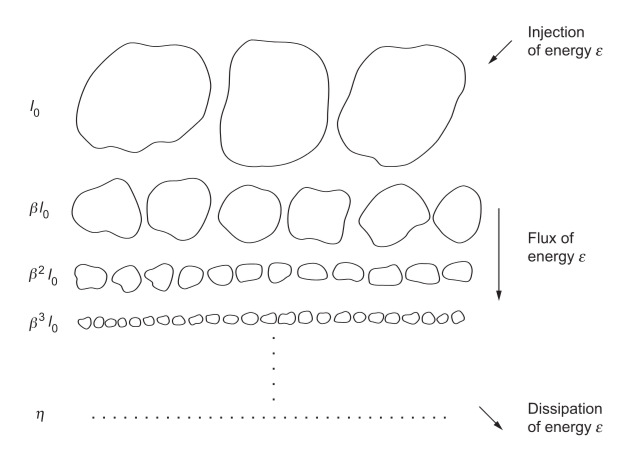
\includegraphics[width=1.2\linewidth]{2/cascade.png}
\caption{Sketch of the Richardson energy cascade process. (Image from Ecke [2005])}
\end{marginfigure}
\begin{center}\begin{minipage}{.8\linewidth}
\emph{‘Big whirls have little whirls that feed on their velocity,
and little whirls have lesser whirls and so on to viscosity.’}
\end{minipage}\end{center}
The nonlinear nature of the governing equations makes it difficult to derive exact results about turbulent flows. It is however possible to derive several useful results starting from plausible assumptions without direct use of the governing equations. This \emph{phenomenological} approach was  pioneered by Kolmogorov [1941a] and Obukhov [1941] following the intuitive ideas of Richardson [1922].
\begin{marginfigure}
\includegraphics[width=1.2\linewidth]{2/autosimilarity.png}
\caption{Illustration of auto-similarity suggested in Richardson 1922}
\end{marginfigure}
It is based on the concept of the energy cascade: energy is fed in the large scales, and a hierarchy of eddies of ever smaller scale is created by successive instabilities. As large eddies break into smaller eddies, the influence of the energy input and the boundary conditions is forgotten and the turbulent flow tends towards local isotropy. At some point, eddies become small enough for dissipation to be important and the cascade terminates. Thus, energy flows continuously from large scales to small scales, where it is dissipated into heat by viscosity in the \emph{dissipative range of scales}. For length scales much smaller than the scale where energy is injected, but also much larger than the dissipative range, the influence of both energy injection and dissipation can be neglected. This range is governed by dissipationless nonlinear energy transfer mediated by the inertial terms of the equations of motion, and is known as the \emph{inertial range}. 

\subsection{Hydrodynamic turbulence: the Kolmogorov-Obukhov theory (K41)}
In the K41 theory, Kolmogorov makes the assumption of locally isotropic time-steady homogeneous fluid turbulence. The time-steady condi tion implies that the energy rate injected into the system, the energy transfer rate and the energy dissipation rate must all be equal on average, while the
local isotropy only holds for very large Reynolds and arises from the fact that
the properties of well developed turbulence at small scales are independent
of the details of the large scales. This has several implications, of which the
most important is that for small scales, or large wave numbers, the turbulence
exhibits \emph{universal} behaviours.
\begin{marginfigure}
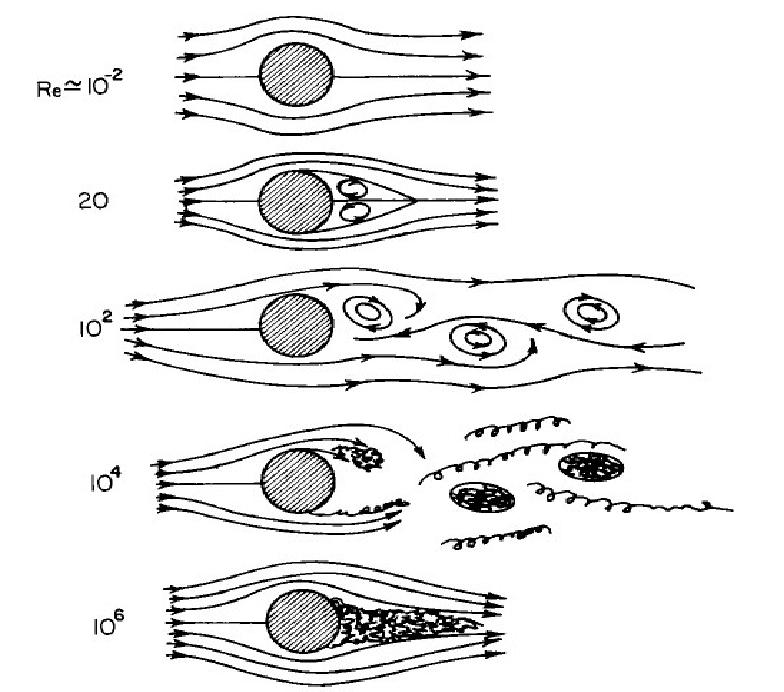
\includegraphics[width=\linewidth]{2/pipeflow.png}
\caption{Schematic view of pipe flow experiments of turbulence at different
Reynolds numbers. Turbulence is fully developed for Reynolds
numbers larger than $10^4$ . (Image from Bohr et al. [1998])}
\end{marginfigure}
Let us concentrate on the properties of a particular eddy lying in the inertial range. The notion of an eddy is not a precisely defined mathematical concept but a loosely defined physical entity: it represents a structure of the turbulent flow localized in space, time and scale. Thus, an eddy is characterized by a length scale $\lambda$ and a velocity scale $\delta u_\lambda$ , which is a typical velocity difference across the distance $\lambda$. From these two quantities we can form a timescale $\tau_\lambda=\lambda/\delta u_\lambda$.
During the cascade process, an eddy of scale $\lambda$ in the inertial range breaks into several smaller eddies of size $\lambda'<\lambda$ under the action of nonlinear instability. These “daughter” eddies go unstable in their turn and break up into the next generation of still smaller eddies. This dissipationless cascade process is repeated until
the eddies produced are small enough for the viscosity to damp the instability that induces the breakdown. 
\begin{marginfigure}
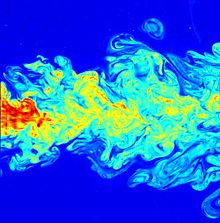
\includegraphics[width=1.1\linewidth]{2/jet.png}
\caption{Turbulent jet observed by laser-induced fluorescence, Fukushima \& Westerweel [2007]}
\end{marginfigure}
For sufficiently high Reynolds numbers, the separation of scales between large scale energy input and small scale dissipation is so large that it is possible to define the inertial range such that the eddies lying there
do not feel the effects of the forcing or the dissipation. In addition, if the inertial range is long enough the
cascade process contains a sufficient number of eddy generations for the large-scale details to be forgotten, leading the small scales towards local isotropy. 

For the inertial range of scales, it is natural to assume that the characteristics of each eddy depend only on the mean energy dissipation rate $\langle\epsilon\rangle$ and the length scale $\lambda$, and not on the scale of the energy input $L$ or the viscosity $\nu$. This assumption is the content of the first hypothesis of similarity of Kolmogorov [1941a]. The energy associated with an eddy of size $\lambda$ is $(\delta u_\lambda)^2$. Assuming that this energy cascades towards smaller scales in the timescale $\tau_\lambda$, we have $\langle\epsilon\rangle=(\delta u_\lambda)^3/\lambda$. Because the energy dissipation rate is, by assumption, a constant quantity independent of scale, we have
\begin{equation}
    \delta u_\lambda\propto\langle\epsilon\rangle^{2/3}\lambda^{2/3}\propto\lambda^{2/3}
\end{equation}
This relation is supported by the 4/5-ths law (71), which implies that the velocity increment should scale as the 1/3-power of the distance. In the inertial range, the structure functions scale as
\begin{equation}
    S_p^L(r)=\langle(\delta u_L(r))^p\rangle\propto(\langle\epsilon\rangle r)^{p/3}
\end{equation}
The transverse structure functions ($L\rightarrow N$) have a similar expression. Since equations (56) and (57) link structure functions and energy spectrum in the power-law case, we can derive 
\begin{equation}
    E(k)\propto\langle\epsilon\rangle^{2/3}k^{-5/3}
\end{equation}
\begin{marginfigure}
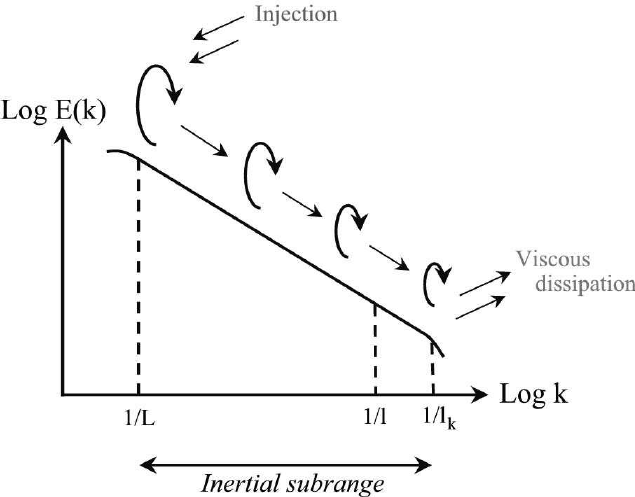
\includegraphics[width=1.1\linewidth]{2/spectrum.png}
\caption{Schematic illustration of production, energy cascade and dissipation in the energy spectrum of turbulence.}
\end{marginfigure}
This expression for the energy spectrum was first derived by Kolmogorov [1941a] and Obukhov [1941]. It was later re-derived indepedently by Onsager [1945] and Heisenberg [1948]. One can use equation (74) to define an eddy Reynolds number 
\begin{equation}
    Re(\lambda)=\frac{\delta u_\lambda\lambda}{\nu}\propto\lambda^{4/3}
\end{equation}
which, as expected, decreases as the scale $\lambda$ decreases: smaller eddies are more and more influenced by viscosity. At the scale $\ell_d$ where $Re(\ell_d ) \sim 1$, viscosity is expected to dominate. This scale can be taken as a representative scale of the dissipative range
\begin{equation}
    \ell_d=\left(\frac{\nu^3}{\langle\epsilon\rangle}\right)^{2/4}
\end{equation}
The above estimate can provide information on the number of active degrees of freedom in a turbulent flow. Assuming that the largest scale is the integral length scale $L_i$, we have
\begin{equation}
    N=\left(\frac{L_i}{\ell_d}\right)^3\propto Re^{3/4}
\end{equation}
Relation (78) for the dissipative scale can equivalently be derived under the assumption that in the dissipative range of scales, the properties of the turbulence should depend only on $\langle\epsilon\rangle$ and $\nu$. This assumption forms the content of the second similarity hypothesis of Kolmogorov [1941a].

\subsection{MHD turbulence and the Iroshnikov-Kraichnan model (IK)}
In incompressible magnetohydrodynamic turbulence, the eddy concept is replaced by the concept of an Alfv\'en wave. Two colliding Alfv\'en waves are deformed by the nonlinear term in such a way that total energy and cross-helicity remain constant, since these quantities are only dissipated by the diffusive terms.
This property allowed Iroshnikov [1964] and Kraichnan [1965] (IK) to construct a phenomenological theory of the inertial range. \sidenote{The MHD equations 
\begin{align*}
\partial_t\mathbf{u}&+(\mathbf{u}\cdot\boldsymbol{\nabla})\mathbf{u}=-\nabla\tilde{p}+\mathbf{j}\times\mathbf{b}+\nu\nabla^2\mathbf{u}\\
\partial_t\mathbf{b}&=\nabla\times(\mathbf{u}\times\mathbf{b}+\eta\nabla^2\mathbf{b}
\end{align*}where $\mathbf{b}=\mathbf{B}=\sqrt{4\pi\rho}$ can be written in a more symmetric form using the Elsässer variables : $\mathbf{z^\pm}=\mathbf{u}\pm\mathbf{b}$
}

The Elsässer equation in the presence of a mean magnetic field $B_0$ can be written 
\begin{equation}
    \partial_t\mathbf{z}^\pm\mp\mathbf{v}_A\cdot\mathbf{z}^\pm+(\mathbf{z}^\mp\cdot\nabla)\mathbf{z}^\pm=-\nabla\tilde{P}+\nu^+\nabla^2\mathbf{z}^\pm+\nu^-\nabla^2\mathbf{z}^\mp
\end{equation}
where $\mathbf{v_A}=\mathbf{B_0}/\sqrt{4\pi\rho}$ is the Alfv\'en velocity defined in terms of the mean field, which can be either a global imposed field, or a local average. 

If the Alfv\'en wave amplitude at a scale $\lambda$ is $\delta u_\lambda$, it changes during collision of two waves by the magnitude of the non-linear term $\delta u_\lambda^2/\lambda$ multiplied by the interaction time $\lambda/{v_A}$ :
\begin{equation}
    \Delta\delta u_\lambda=\frac{\delta u_\lambda^2}{v_A}
\end{equation}
If one further assumes that collisions change the energy of the waves as a random walk, the number of collisions required to deform each wave considerably is 
\begin{equation}
    N=\left(\frac{\delta u_\lambda}{\Delta\delta u_\lambda}\right)^2=\left(\frac{v_A}{\delta u_\lambda}\right)^2
\end{equation}

The timescale of a such cascade would thus be $\displaystyle\tau_{IK}=\frac{N\lambda}{v_A}=\frac{\lambda v_A}{\delta u_\lambda^2}$.
Assuming a constant energy flux through the inertial range $\langle\epsilon\rangle=\delta u_\lambda^2/\tau_{IK}$ gives the scaling
\begin{equation}
    \delta u_\lambda\propto(\langle\epsilon\rangle B_0\lambda)^{2/4}
\end{equation}
The prediction for the energy spectrum,
\sidenote{numerical and analytical studies of incompressible MHD turbulence,
where the cascade is mediated by Alfv\'en fluctuations, show that the different
scaling exponents for the power spectra might depend upon the strength of
the turbulence, the strength of the background field, $B_0$, and anisotropy.
Specifically, it has been observed that introducing anisotropy to MHD models
of turbulence, the power spectrum scales as $\sim k^{-2}$ for weak turbulence [e.g.
Galtier et al., 2000] and $\sim k^{-5/3}$ - i.e. the Kolmogorov spectrum - for strong
turbulence [e.g., Higdon, 1984; Goldreich and Sridhar, 1995] with respect to the
background magnetic field. In particular, Goldreich and Sridhar [1995] showed
that magnetic and velocity field perturbations only occur perpendicular to $B_0$
leading to the following relationship $k_\parallel=k_\perp^{-2/3}\ell_0^{-1/3}$, where $\ell_0$ is the outer or energy injection scale. Considering the turbulence cascade picture, this could be seen as elongated eddies - i.e. “rope-like” or “sheet-like” structures - along the direction of $B_0$.}following similar arguments than for K41, is thus
\begin{equation}
    E(k)\propto C_{IK}(\langle\epsilon\rangle B_0)^{2/2}k^{-3/2}
\end{equation}
And the dissipative scale is
\begin{equation}
    \ell_d^{IK}=\left(\frac{B_0\eta^2}{\langle\epsilon\rangle}\right)^{2/3}
\end{equation}


\subsection{Compressible turbulence}

From the point of view of phenomenology, an important difference between incompressible and compressible turbulence is the absence, in the compressible case, of a quadratic conserved quantity which would allow the construction of a cascade argument. In incompressible turbulence this role is played by the kinetic energy $1/2\langle\mathbf{u}^2\rangle$ which is exactly conserved by nonlinear interactions involving triads of wavenumbers. 

In compressible turbulence the conserved quantity is the total energy $\langle e+1/2\rho\mathbf{u}^2\rangle$ which involves the internal
energy of the gas and cannot be obviously related to the statistics of the velocity field. Another complicating factor is that nonlinear interactions in compressible turbulence are fundamentally more complex due to the presence of the density field. Even in the case of isothermal turbulence, where the conserved quantity is $\langle1/2\rho\mathbf{u}^2\rangle$, the cubic nonlinearity due to the presence of the density field complicates things considerably.

Theoretical results in compressible turbulence are even scarcer than incompressible turbulence. Galtier and Banerjee [2011] have derived an exact expression, analogous to the 4/5ths law, for the third order structure function in isothermal turbulence. Banerjee and Galtier [2013] have generalized this result for isothermal magnetohydrodynamic turbulence.

\section{Intermittency and self-similarity|multifractality}
All the phenomenological theories presented in the previous section are built on the assumption that the energy dissipation rate $\epsilon(x)$ is uniformly distributed in space. Both experiments [Batchelor and Townsend, 1949, Grant et al., 1962, Anselmet et al., 1984] and numerical simulations [Siggia, 1981, Kerr, 1985, Vincent and Meneguzzi, 1991] have shown that this is not the case: in fact, the energy dissipation rate is concentrated on a few intense structures separated by large quiescent regions, a property known as intermittency.
The property of intermittency has obvious important practical consequences for the heating in a turbulent flow, but it also has important theoretical consequences for the general scaling properties of the turbulence.

\subsection{Definitions and framework}

Let us focus on the longitudinal component of a turbulent velocity field $u_L(x)$. The property of intermittency can be quantified if one considers the random variable
\begin{equation}
    \theta(r)=\frac{\delta u_L(\mathbf{x},\mathbf{r})}{(\langle\epsilon\rangle r)^{2/3}}=\frac{u_L(\mathbf{x}+\mathbf{r}-u_L(\mathbf{x})}{(\langle\epsilon\rangle r)^{2/3}}
\end{equation}
where homogeneity and isotropy of the velocity field have been assumed. Under the assumptions leading to K41, the probability density function of the random variable $\theta(r)$ should be independent of the scale r: the velocity field is \emph{self-similar}. Perhaps the most well-studied example of a self-similar random function is Brownian motion, a realization, which is represented in figure \ref{fig:2-brown}.
\begin{marginfigure}[-10cm]
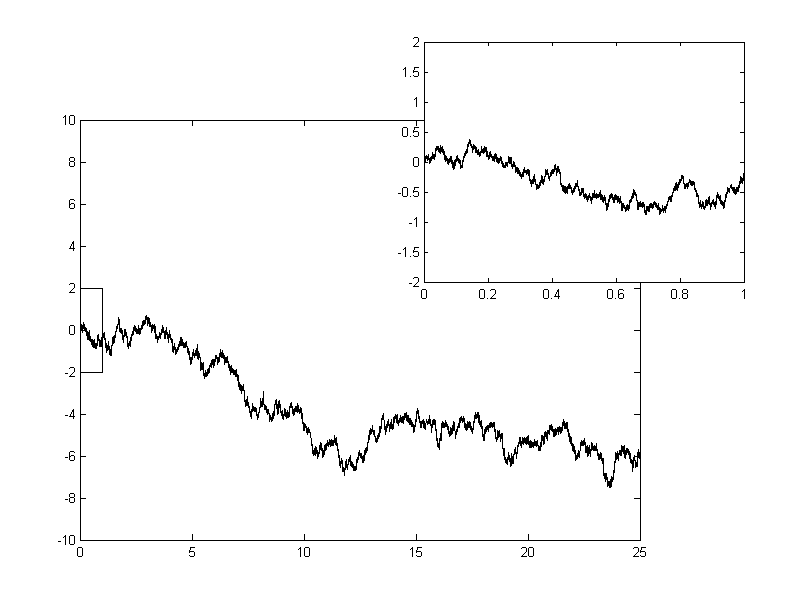
\includegraphics[width=1.3\linewidth]{2/brown.png}
\caption{A realization of one-dimensional Brownian motion. ”Wiener process zoom”}
\label{fig:2-brown}
\end{marginfigure}Here it is intuitively clear that the statistical properties of the curve do not depend on scale.

For an intermittent velocity field however, this is no longer the case: as smaller separations $r$ are consid ered, the tails of the distributions corresponding to extreme velocity bursts become increasingly important. For example in many cases the distribution $p(\delta u_L(x,r))$ is very close to Gaussian for large $r$ but assumes a very different form, such as a stretched exponential for small r. 
\begin{marginfigure}[-3.5cm]
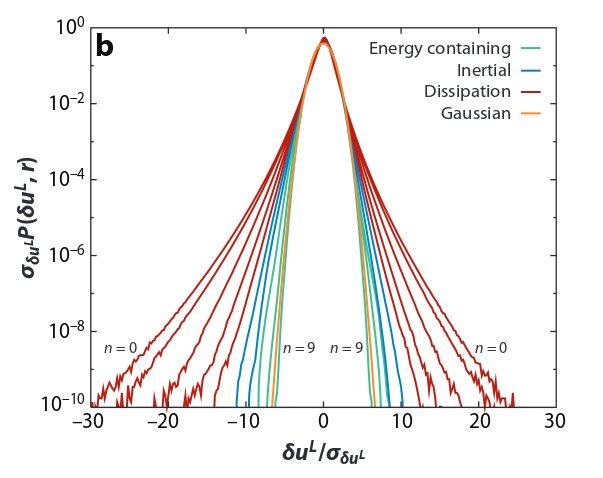
\includegraphics[width=\linewidth]{2/pdf.png}
\caption{Pdf of the longitudinal velocity increment from a high resolution incompressible hydrodynamical
simulation for various separations $r_n = 2 n \delta x$, $\delta x$ being the distance between grid points in the simulations. (from Ishihara et al. [2009])}
\label{fig:2-ishihara}
\end{marginfigure}This can be seen clearly in figure \ref{fig:2-ishihara}, where the pdf of the longitudinal velocity increment from a high resolution incompressible hydrodynamical simulation is shown for various separations. For a function that exhibits no intermittency, the non-dimensional ratios\sidenote{We will use longitudinal structure functions for definiteness, although there is no distinction between longitudinal and
transverse structure functions in the context of this chapter.}
\begin{equation}
    F(r)=\frac{S_L^{2p}(r)}{(S_L^p(r))^2}
\end{equation}
are independent of scale: there is no statistical difference between large and small scales. For an intermittent function, by contrast, there is by definition much more extreme bursts in the small scales than in the large scales, and thus the ratios $F(r)$ are expected to grow with decreasing $r$:
\begin{equation}
    F(r)\propto\left(\frac{L_i}{r}\right)^\delta
\end{equation}
This is because the structure functions $S^{2p}(r)$ in the nominator are of higher order than those in the denominator, and thus sample the tails of the probability distribution of the velocity increment corresponding to extreme events. For an intermittent function, these tails become stronger and stronger at small increments leading to a faster increase of the quantity $S^{2p}(r)$ in comparison with $(S^p(r))^2$. Thus the introduction of the
property of intermittency breaks the self-similarity of the velocity field by introducing the integral length scale $L_i$ in the scaling of the statistics.
The phenomenological theories presented in the previous are clearly self-similar. In K41 for example, the structure functions scale as
\begin{equation}
    S_p^L(r)\propto r^{p/3}
\end{equation}
which implies that F (r) is constant. These phenomenological theories are therefore incompatible with intermittency, with this geometrical approach. 
Fractal geometries, however, because of their unique scaling properties can reconcile the statistical and phenomenological views of turbulence, with the structures and shapes emerging from observations. Their introduction, by fractal dimensions, can be stated very simply :

Let us assume a $\ell_n$ sized structure occupying a  $\ell_n^3$ portion of space.
Admitting a scaling factor $b$, this structure will give birth to $N$ structures, sized $\ell_{n+1}$, each of these sub-structures filling a $\ell_{n+1}$ volume.

This descriptive approach is closely similar to that of the notion of intermittency, primairly developped in turbulence descriptions :

\begin{itemize}
    \item Without intermittency\sidenote{Intermittent behaviour is commonly observed in fluid flows that are turbulent or near the transition to turbulence. In highly turbulent flows, intermittency is seen in the irregular dissipation of kinetic energy. It is also seen in the irregular alternation between turbulent and non-turbulent fluid that appear in turbulent jets and other turbulent free shear flows. In pipe flow and other wall bounded shear flows, there are intermittent puffs that are central to the process of transition from laminar to turbulent flow. Intermittent behavior has also been experimentally demonstrated in circuit oscillators and chemical reactions.}, the entire available space is filled by the N structures of dimension $\ell_{n+1}$. i.e., $$N=b^3$$
    \item intermittency, is when all the new substructures are not capable of filling the entire space, i.e., $$N<b^3$$
\end{itemize}

This global cascade process is called ``fractal'' provided this number is independant of the considered step $n$. At every evolutive step, the volume ratio will hold
\begin{equation}
    \frac{V_{n+1}}{V_n}\sim\frac{N}{b^3}
\end{equation}
The fractal dimension of the structures in this process can therefore befined as 
\begin{equation}
    N=b^D\;\;\text{i.e.}\;\;D=\log_b{N}
\end{equation}
Thus
\begin{equation}
        \frac{V_{n+1}}{V_n}\sim b^{D-3}
\end{equation}

Technical details about the intervention of fractal dimensions, fractal structures and objects are given in Appendices : K/H Fractals, Internal similarity law and multifractality.

\subsection{Scaling properties of the dissipation field}
The refined similarity hypothesis\sidenote{The measures of intermittency of the velocity field, expressed by the scaling of the structure functions $S_p^L(r)$, can be related to the intermittency characteristics of the dissipation field $\epsilon(x)$. Obukhov [1962] suggested
that the mean energy dissipation rate $\langle\epsilon\rangle$ could be replaced by 
$$\epsilon_r=\frac{3}{4\pi r^3}\int_B\epsilon(\mathbf{x})d\mathbf{x}$$ which is the energy dissipation rate averaged over a sphere $B$ of radius $r$.
Are then defined the time scale $T_r=r^{2/3}\epsilon_r^{-1/3}$, the velocity scale $U_r=(r\epsilon_r)^{2/3}$, the scale-dependant Reynolds $Re=r^{4/3}\epsilon^{2/3}/\nu$, and the dissipation scale $\ell_r^d=\nu^{3/4}\epsilon^{-1/4}$. Assuming $\ell_r^d<<r<<L_i$, the scaling exponents of the dissipation field and of the structure functions can be bridged
$$S_p^L(r)\propto\langle\epsilon\rangle^{p/3}r^{\zeta_p^L}\quad;\quad \zeta_p^L=p/3+\tau_p/3$$, where $\tau_p$ is the scaling exponent of the dissipation field} suggests that the K41 theory is only a first approximation because it ignores fluctuations in the energy dissipation rate. Thus K41 is only a mean field theory of turbulence and fluctuations in the dissipation rate will introduce at least one more universal scaling exponent. In this context, the most simple relevant correlation is
\begin{equation}
    \langle\epsilon(\mathbf{x}+\mathbf{r})\epsilon(\mathbf{x})\rangle=\frac{1}{2}\frac{d^2}{dr^2}(r^2\langle\epsilon_r\rangle)
\end{equation}
where the right hand side follows from homogeneity and the definition of $\epsilon_r$. For $r$ in the inertial range of scales, it is natural to assume that this correlation function scales as a power of $r$. Assuming further that the viscosity plays no role at these scales, we expect, 
\begin{equation}
    \langle\epsilon(\mathbf{x}+\mathbf{r})\epsilon(\mathbf{x})\rangle\propto\langle\epsilon\rangle^2\left(\frac{L_i}{r}\right)^\mu
\end{equation}
Thus, the fluctuations of the dissipation field introduce a new scaling exponent $\mu$. For incompressible hydrodynamic turbulence, the value of $\mu$ found in experiments and numerical simulations is $0.20 \pm 0.05$ [Anselmet et al., 2001].
As an example of how the exponent $\mu$ can enter the scaling of the velocity field, let us suppose that indeed in the inertial range $\epsilon_r$ scales as expected and the structure functions $S_L^p(r)$ scales as (89). the refined similarity hypothesis implies that 
\begin{equation}
    \zeta_6^L=3-\mu
\end{equation}
The scaling properties of the energy dissipation rate can be characterized in more details by introducing the notion of \emph{multifractality} [Frisch and Parisi, 1985, Paladin and Vulpiani, 1987]. The energy dissipation field is said to be multifractal if it exhibits the scaling
\begin{equation}
    \frac{\epsilon_r(\mathbf{x}}{\langle\epsilon\rangle}\propto\left(\frac{r}{L_i}\right)^{\alpha-1}
\end{equation}
for all points $x$ lying in a set $\mathcal{D}_\alpha$ which has fractal dimension $\dim \mathcal{D}_\alpha = F(\alpha)$. Thus, a multifractal dissipation
field has singularities of exponent $\alpha-1$ on sets of dimensions $F(\alpha)$. The function $F$ is called the spectrum of singularities of the multifractal field. 
For a three-dimensional turbulent flow, the probability of a randomly chosen sphere centered at the point $\mathbf{x}$ with a radius equal to $r$ to lie in a given set $\mathcal{D}_\alpha$ scales as [Frisch, 1995]
\begin{equation}
    \mathbb{P}[x\in\mathcal{D}_\alpha]\propto\left(\frac{r}{L_i}\right)^{3-F(\alpha)}
\end{equation}
The moment of dissipation is thus given by the integral 
\begin{equation}
    \langle\epsilon_r^q\rangle=\langle\epsilon\rangle^q\int_{\alpha_{min}}^{\alpha_{max}}\left(\frac{r}{L_i}\right)^{q(\alpha-1)+3-F(\alpha)}
\end{equation}
By a steepest-descent argument [Bender and Orszag, 1999], the above integral yelds the dissipation scaling exponent, called $\tau_q$ :
\begin{equation}
    \tau_q=\min_\alpha\{q(\alpha-1)+3-F(\alpha)\}
\end{equation}
An important consequence of multifractality which is apparent in the above relation is that the scaling exponent $\tau_q$ becomes in general a nonlinear function of the order. Through the bridge relation, this implies that the longitudinal structure function scaling exponents $\zeta_p^L$ are also a nonlinear function of $p$.
This is to be contrasted with the phenomenological theories of section 4 which all predict a linear relation between $p$ and $\zeta_p^L$ , but also with the unifractal beta model of Frisch et al. [1978].

The above definition of multifractality assumes that singularities are indeed present in the dissipation field, a fact that is far from obvious based on the current understanding of the Navier-Stokes equation [Gallavotti,1992, Foias et al., 2002]. One can circumvent this difficulty by adopting the following probabilistic definition of multifractality [Frisch, 1995]: the dissipation field is said to be multifractal if there is a function $F(\alpha)$
which maps real scaling exponents $\alpha$ to scaling dimensions $F \leq 3$ such that for any $\alpha$ we have
\begin{equation}
    \lim_{r\rightarrow0}\frac{\ln\mathcal{C}_r(r^{\alpha-1}}{\ln r}=3-F(\alpha)
\end{equation}
where $\mathcal{C}_r(\epsilon)$ is the cumulative distribution function of the energy dissipation rate $\epsilon_r$. In addition to avoiding the unnecessary assumption of the existence of singularities in the dissipation field, the above probabilistic definition leads to the interpretation of intermittency in terms of large deviations theory [Frisch, 1995], which will not be presented here.

\newthought{The scaling} laws can be grouped using a universal constant $\chi$ and the integral scale of turbulence $\ell_0$ :\begin{fullwidth}
\begin{align}
    (\text{Two-thirds law})\quad\quad&S_2(\ell)\sim\langle\epsilon\rangle^{2/3}\ell^{2/3}\left(\frac{\ell}{\ell_0}\right)^{\chi/9}\\
    (\text{Five-thirds law})\quad\quad&E(k)\sim\langle\epsilon\rangle^{2/3}k^{-5/3}(k\ell_0)^{-\chi/9}\\
    (\text{Moments' law})\quad\quad&S_p(\ell)\sim\langle\epsilon_\ell^{2/3}\rangle\ell^{p/3}\sim\langle\epsilon\rangle^{p/3}\ell^{p/3}\left(\frac{\ell_0}{\ell}\right)^{\chi p(p-3)/18}
\end{align}
\end{fullwidth}
Besides the K-O62 model, numerous models have been developed in order to include intermittency effects in the turbulence cascade, some of which employ a (multi)fractal approach to the statistical description of fully developed turbulence. The use of the fractal geometry arises from the energy cascade picture: analogously to a fractal, a single eddy can be seen as a rough
part or a fragmented geometric shape that can be subdivided into parts, the daughter eddies, each of which is a reduced size of the mother eddy [Seuront et al., 1999]. 

When intermittency phenomena occur, not all daughter eddies are generated producing therefore ‘gaps’ in the hierarchy of cascading eddies leading to a non-uniform distribution in space (or time) of the eddies. As a consequence of this, the eddies are no longer space-filling and the energy
dissipation rate within the inertial range depends on scale $\ell$.\sidenote{There are several definitions of intermittency in literature, some of which threat the non-constant energy dissipation rate and the non-space-filling nature of turbulence separately.}

\subsection{Random Cascade model (unifractal-$\beta$)}

Let us consider a turbulent flow inside a cube of side $\ell_0$ in which the energy dissipation rate is uniform, equal to $\langle\epsilon\rangle$. In a random cascade model, this uniform average value represents the “mother eddy” of generation $n = 0$. The eddies of the next generation $n = 1$ are obtained by subdividing the cube into eight equal
sub-cubes of side $l_1 = l_0 /2$\sidenote{We here take 2 for simplicity and visualisation, but it is strictly identical to writing $\ell=\ell_0r^n$}. In each new sub-cube, the value of the energy dissipation rate is defined as the product of the value corresponding to the previous generation with a chosen random variable $W$, which has the following properties:
\begin{equation}
    W\leq0\quad;\quad\langle W\rangle=1\quad;\quad \langle W^q\rangle<\infty,q>0
\end{equation}
\begin{marginfigure}
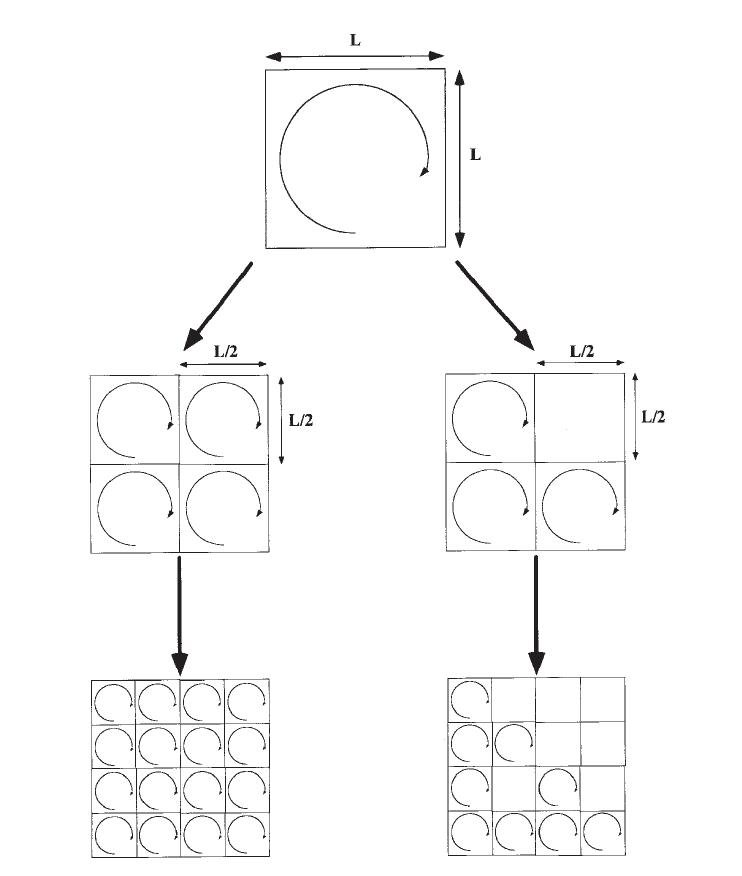
\includegraphics[width=1.2\linewidth]{2/turbulentcascade1.png}
\caption{Sketch of a turbulent cascade: non-intermittent case (left) and
intermittent, mono-fractal case (right).}
\label{fig:2-fcascade}
\end{marginfigure}
The model is defined by taking $\beta$ the fraction of the $2^n$ daughter eddies of size $\ell=\ell_02^{-n}$ produced. Each of these eddies is characterized by a uniform value of the energy dissipation rate which is equal to
\begin{equation}
    \epsilon_\ell=\langle\epsilon\rangle\prod_{i=1}^nW_i
\end{equation}
With the $\beta$ parameter, we have
\begin{equation}
    W=\begin{cases}
    1/\beta & \text{with probability } \beta\\
    0 &  \text{with probability } 1-\beta\end{cases}
\end{equation}
Which means that the moments of $\epsilon_\ell$ are given by
\begin{equation}
    \langle\epsilon_\ell\rangle=\langle\epsilon^q\rangle\left(\frac{\ell}{\ell_0}\right)^{\tau_q}
\end{equation}
Where
\begin{align}
    \tau_q&=-\log_2\langle W^q\rangle = -(1-q)\log_2\beta\\
    \zeta_p&=\frac{p}{3}-\left(1-\frac{p}{3}\right)\log_2\beta
\end{align}

However, the phenomenology of turbulent cascades is rather more complex and mono-fractal models, like the $\beta$-model, do not take into account how the activity of turbulence becomes more and more inhomogeneous as we go to smaller and smaller scales\sidenote{From an experimental point of view, mono-fractal models are inadequate to describe
intermittent turbulence since they lead to a linear dependence of $\zeta(p)$ on $p$, while experiments tend to agree on a quadratic dependance, or at least, non-linear}. 
\begin{figure}[t]
\centering
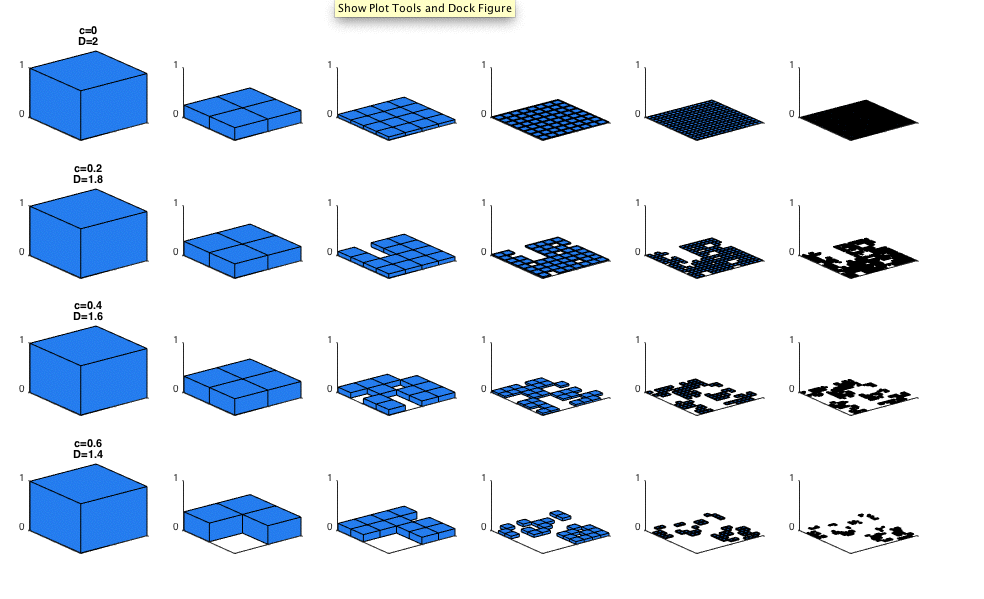
\includegraphics[width=\linewidth]{2/betamodel.png}
\caption{betamodel illustration................}
\end{figure}
Figure \ref{fig:2-fcascade} shows the phenomenology of the turbulent cascade with (right) and with-
out (left) intermittency effects. The intermittent case here shown refers to a
mono-fractal description of intermittency, such as that used in the $\beta$-model.
As we can see, mono-fractal models only consider the case for a daughter eddy
of a fixed size to be generated or not. It does not consider the intermediate
case for which eddies of similar but different sizes can be generated. The latter
case would be instead taken into account in a multifractal description of the
turbulent cascade as can be seen in Figure \ref{fig:2-mfcascade}. 
\begin{marginfigure}
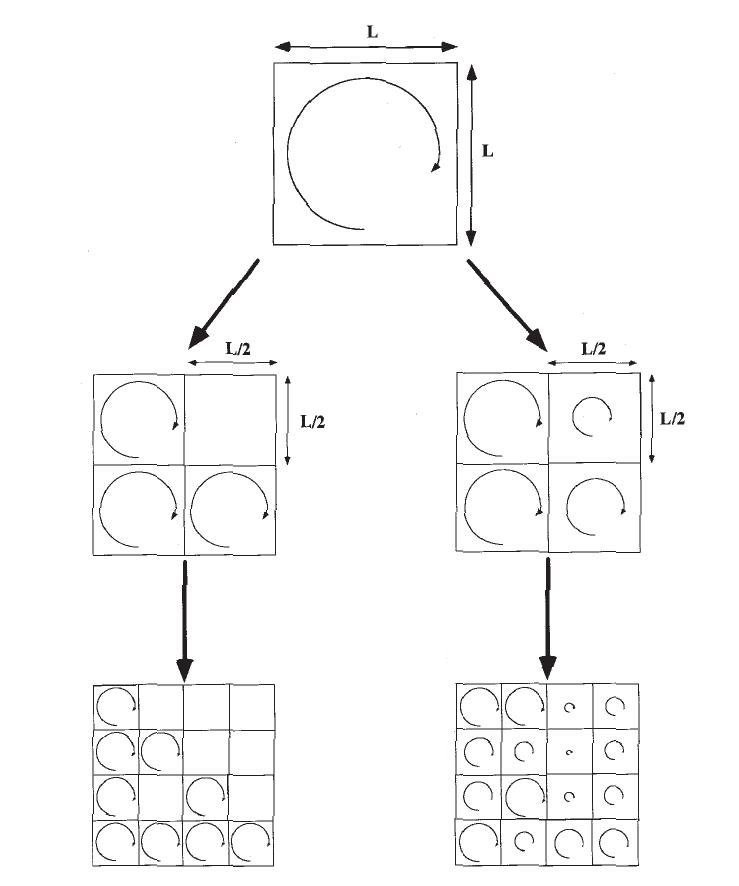
\includegraphics[width=1.2\linewidth]{2/multifractalcascade.png}
\caption{Multifractal description of the turbulent cascade: mono-fractal
description (left) versus multi-fractal description (right)}
\label{fig:2-mfcascade}
\end{marginfigure}

Such multifractality is generated by considering probability density functions for random variable $W$. These models are purely phenomenological, as they do not deduce intermittency properties directly from the governing equations but use instead plausible physical assumptions for the cascade process.

\subsection{Log-Normal model (K-O62)}
The assumption of a log normal PDF is natural, considering various PDF observations (notably for filaments, e.g. Henebelle, André, Arzoumanian 07,08,10,11,13,17) and the logarithm of the dissipation $\epsilon_\ell$ :
\begin{equation}
    \ln\epsilon_\ell=\ln\langle\epsilon\rangle+\sum_{i=1}^n\ln W_i
\end{equation}
Hence for small scales $\ell$ the logarithm of $\epsilon_\ell$ is equal to the sum of a large number of independent identically distributed random variables. The central-limit theorem implies that the random variable $\ln\epsilon_\ell$ is normally distributed, hence the log-normal probability density function for $\epsilon_\ell$. 
Since the sum of Gaussian variable is a Gaussian variable, we can use the formalism of large deviations theory [Frisch, 1995] to compute the singularity spectrum of the dissipation field:
\begin{equation}
    F(\alpha)=3-\frac{(\alpha-1-\mu/2)^2}{2\mu}
\end{equation}
where $\mu$ is the same quantity that appears in the scaling of local energy dissipation rate $\epsilon_r$ in equation (94). Thus the values of the scaling exponents predicted by the log-normal model are
\begin{align}
\tau_q&=\frac{\mu}{2}(q_q^2)\\
\zeta_p^L&=\frac{p}{3}+\frac{\mu}{18}(3p-p^2)
\end{align}
The log-normal model predicts a nonlinear relation between the scaling exponents and the
order of the moment, and thus exhibits multifractal scaling.\sidenote{However, this model violates the []Novikov 1971] inequality, due to the non-conservative nature of the cascade. For certain values, the spectrum $F(\alpha)$ becomes negative, which [Mandelbrot, 1972] stem from the invocation of the central limit theorem, which completely ignores large
deviations}

\begin{figure}[h]
\centering
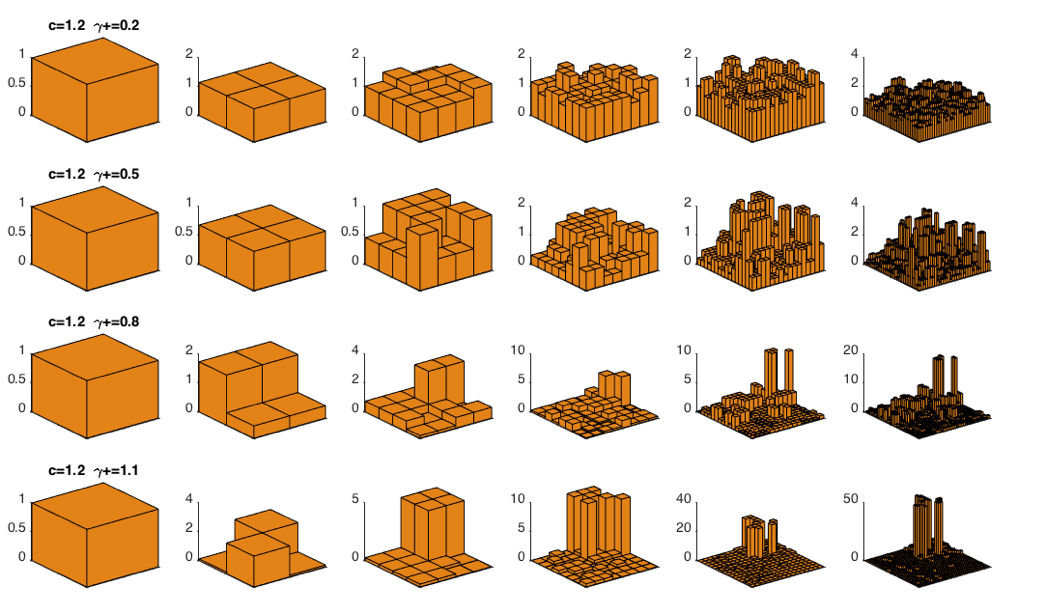
\includegraphics[width=\linewidth]{2/alphamodel.png}
\caption{alphamodel illustration................}
\end{figure}

\subsection{Log-Poisson model (She-Leveque 98)}
A very successful intermittency model was introduced by She and Leveque [1994b] for the case of incompressible hydrodynamic turbulence. The model was later generalized by Grauer et al. [1994] and Politano and Pouquet [1995] for incompressible magnetohydrodynamic turbulence and by Boldyrev et al. [2002] for compressible hydrodynamic turbulence. Dubrulle [1994], She and Waymire [1995] reinterpreted the model in terms of log-Poisson statistics. Apart from being successful in reproducing experimental, observational and numerical results, this model is unique in incorporating geometrical information about dissipative structures.

The energy dissipation field averaged over a ball of radius $\ell\epsilon_\ell$ is characterized by a hierarchy of fluctuation structures $\epsilon_\ell^{(p)}$, $p=0,1,2,\dots$ defined by the ratio of successive dissipation moments :
\begin{equation}
    \epsilon_\ell^{(p)}=\frac{\langle\epsilon_\ell^{p+1}\rangle}{\langle\epsilon_\ell^p\rangle}
\end{equation}
The first structure of the hierarchy corresponds to the mean energy dissipation rate $\langle\epsilon\rangle$, and the "last" $\epsilon_\ell^{(\infty)}$ corresponds to the small scale dissipative structures, assumed to be \emph{vortex filaments}.

It is known from numerical experiments [Siggia, 1981, Kerr, 1985, Vincent and Meneguzzi, 1991] that dissipation of high intensity displays a certain degree of coherence in space, typically organizing itself in filamentary structures [Moisy and Jiménez, 2004]. The motivation behind the original formulation of the log-Poisson model is that these coherent structures can have scaling properties which are captured by the hierarchy $\epsilon_\ell^{(p)}$.
The first structure of the hierarchy is scale independent by definition, as it is equal to the mean energy dissipation rate used in the context of K41 to predict normal, non-anomalous scaling. Here, anomalous scaling is introduced by the divergent scaling dependence of $\epsilon_\ell^{(\infty)}$ as $ \ell\rightarrow0$ due to the presence of filamentary
structures of high dissipation. The last structure in the hierarchy can be estimated dimensionally :
\begin{equation}
    \epsilon_\ell^{(\infty)}=E^{(\infty)}/t_\ell
\end{equation}
where $E$ is the kinetic energy available to the cascade\sidenote{Mostly supernovae explosions, then stellar winds, protostellar outflow.. c.f. Section 6} and $t_\ell$ the timescale.
Assuming that the nonlinear processes that determine the timescale of the cascade are homogeneous in space, irrespective of the presence of structures of high dissipation implies a K41 scaling for the timescale
\begin{equation}
    t_\ell\propto\langle\epsilon\rangle^{2/3}\ell^{2/3}
\end{equation}
If we further assume that kinetic energy dissipated by the most intense structures $E_\ell^{(\infty)}$ is independent of scale and equal to the large-scale kinetic energy $1/2U^2$, we obtain the scaling
\begin{equation}
    \epsilon_\ell^{(\infty)}=\langle\epsilon\rangle\left(\frac{\ell}{L_i}\right)^{-2/3}
\end{equation}
Thus, such an anomalous $\ell^{2/3}$ scaling for the energy flux imply that as $p\rightarrow\infty$, $\tau_{p+1}-\tau_p\rightarrow2/3$, ie
\begin{equation}
    \tau_p=-\frac{2}{3}p+C_0 \quad;\quad p\rightarrow\infty
\end{equation}
$C_0$ can be interpreted as the co-dimension of the most intense dissipative structures.
Assuming that these structures are filaments\sidenote{Here we take the dimension to a filament to be around 1. In fact, \emph{Herschel} observations tend to use a slightly higher dimension,between 1.25 and 1.3}, we have $C_0=2$, and $\tau_p=2/3p+2$. 

The dissipation intensities $\epsilon_\ell^{(p)}$ characterize less intense dissipative structures and their scaling with $\ell$ can provide a measure of how singular these structures are. The less intense structures are assumed to be the results of the same dynamics which form the most intense structures $\epsilon_\ell^{(\infty)}$, but fail to accomplish this high degree of coherence because of background disorder. In physical space, structures of higher intensity are likely to be surrounded by structures of lower intensity. Similarly in time, structures of lower intensity tend to come first. These facts suggest that there may be a relation between
the intensities $\epsilon_\ell^{(p)},~\epsilon_\ell^{(p+1)}$  and $\epsilon_\ell^{(\infty)}$. The relation proposed by She and Leveque [1994b] as a consequence of \emph{some hidden (statistical) symmetries of the Navier-Stokes equations reads} : 
\begin{equation}
    \epsilon_\ell^{(p+1)}\propto\Big(\epsilon_\ell^{(p)}\Big)^\beta\Big(\epsilon_\ell^{(\infty)}\Big)^{1-\beta}\quad,\quad0<\beta<1
\end{equation}
The proportionnality constants are scale-independant, but non-universal. This gives 
\begin{equation}
    \tau_{p+2}-(1-\beta)\tau_{p+1}+\beta\tau_p+\frac{2}{3}(1-\beta)=0
\end{equation}
The solution must satisfy the boundary conditions $\tau_0=0$ which follows from the assumption of finite dissipation in the limit of zero viscosity, and $\tau_1=0$ which follows from the $4/5$ths law and the bridge relation. 
The scaling exponents of the dissipation moments are thus
\begin{align}
    \tau_p&=-\frac{2}{3}p+2\times\bigg[1-\left(\frac{2}{3}\right)^p\bigg]\\
    \zeta_p^L&=\frac{p}{9}+2\times\bigg[1-\left(\frac{2}{3}\right)^{p/3}\bigg]
\end{align}
And the energy spectrum is predicted as
\begin{equation}
    E(k)\propto k^{29/9+2\times(2/3)^{2/3}}
\end{equation}
The intermittency exponent $\mu$ is predicted at $\mu=2/9$. 
\begin{marginfigure}
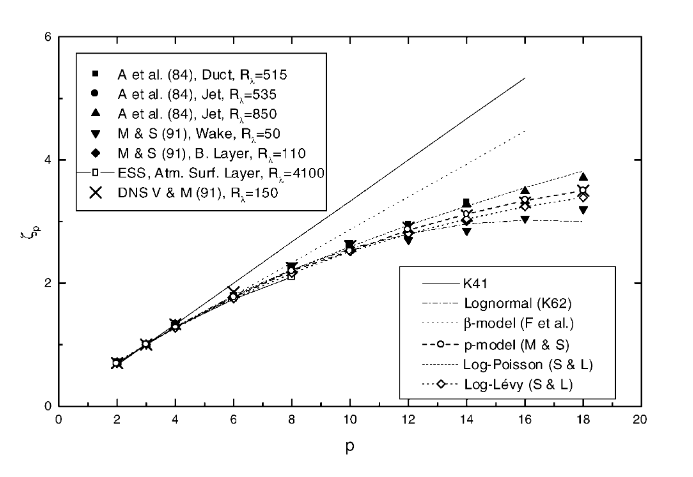
\includegraphics[width=1.2\linewidth]{2/intermittency.png}
\caption{Comparison of experimental data with the predictions of the structure function scaling exponents of various intermittency models (from Anselmet et al. [2001])}
\label{fig:2-intermodels}
\end{marginfigure}
The log-Poisson model has met considerable success in predicting experimental, observational and numerical results Anselmet et al. [2001]. Three important ingredients that render the model unique are the postulated scaling relation (2.189) which attempts to capture the nonlinear dynamics of the cascade, the consideration of the filamentary character of the most intense dissipative structures and the assumption of a divergent scaling law for the energy flux. This success of the log-Poisson model is illutrated in figure \ref{fig:2-intermodels}, which shows a comparison of experimental data with the predictions of the structure function scaling exponents of various intermittency models.

\newthought{For MHD turbulence}, ie, taking into account the inertial interactions of Alfvén
waves, Grauer et al. [1994] and Politano and Pouquet [1995] have extended the log-Poisson model. The refined similarity hypothesis becomes 
\begin{equation}
    \epsilon_\ell=\propto\frac{(\delta z(\ell))^g)}{\ell B_0^{g+3}}
\end{equation}
Where $\delta z(\ell)$ is the Elsässer increment, $g$ the inverse of the scaling exponent in the inertial range ($\delta z(\ell)\propto\ell^{2/g}$ and $B_0$ the quasi-uniform field that guides the Alfvén waves. For IK phenomenology, $g=4$\sidenote{However, for K41, $g=3$}. Assuming the scaling
\begin{equation}
    \epsilon_\ell^{(p+1)}=A_p^B((\epsilon_\ell)^{(p)})^{\beta_B}((\epsilon_\ell)^{(\infty)})^{1-\beta_B}\quad;\quad0<\beta_B<1
\end{equation}
for the dissipation hierarchy, and 
\begin{equation}
    t_\ell\propto\ell^{\left(1-\frac{1}{g}\right)}
\end{equation}
for the time scale of the cascade domain, we have
\begin{equation}
    \tau_p=-\frac{p}{g}+(C_0^B)^{1-p}\left(1-\frac{1}{g}\right)^p
\end{equation}
for the dissipation exponents and
\begin{equation}
    \zeta_p^B=\frac{p}{g}\left(1-\frac{2}{g}\right)+C_0^B\left(1-\left(1-\frac{2}{gC_0^B}\right)\right)^{p/g}
\end{equation}
where the co-dimension $C_0^B$ is given by :
\begin{equation}
    C_0^B=\frac{1-g}{1-\beta_B}
\end{equation}
Thus the model contains two free parameters: the inertial range scaling exponent $g$ and the co-dimension of the dissipative structures $C_0^B$ . In magnetohydrodynamic turbulence, the co-dimension $C_0^B \sim 1$ as most of the dissipation occurs in quasi two-dimensional sheet-like structures. The exponent parameter $g$ can be either 3 for K41 scaling or 4 for IK scaling. This generalization of the log-Poisson model has met considerable success in predicting results of numerical simulations [Müller and Biskamp, 2000] and solar wind observations Politano and Pouquet [1995].

\newthought{For compressible} turbulence, Boldyrev et al. [2002] assumed that the inertial range of compressible magnetohydrodynamic turbulence is governed by K41 scaling leading to the choice g = 3. The co-dimension is taken equal to 1 because the dissipation is assumed to take place in shocks, which are two dimensional structures. This “Kolmogorov-Burgers” model, which is identical with the model used in the numerical study of Müller and Biskamp [2000] in the context of incompressible magnetohydrodynamics, has been successfully compared against numerical simulations of isothermal hydrodynamic and magnetohydrodynamic compressible turbulence [Padoan et al., 2004, Kritsuk et al., 2007].

